% todo: pensar em colocar uma parte falando sobre o método dos mínimos quadrados
\part{Teoria}
	\chapter{Reologia}
		\section{Fundamentos}
		
		% todo: Pensar se eu devo colocar que vem do grego rheos, corrente/rio/fluxo e logia, estudo/ciência
		% todo: pensar se eu devo falar que foi cunhado pelo Prof. Bingham em 1929
		A reologia é a área ciência que estuda o fluxo e a deformação da matéria. Para causar um fluxo ou deformação, é necessário que uma força externa seja aplicada ao corpo. Reagindo à essa força, o material se comporta de tal maneira que algumas de suas características estruturais podem ser inferidas. Isso é feito intuitivamente por qualquer pessoa, por exemplo, ao apertar uma fruta para determinar sua firmeza e assim, se ela está apropriada para consumo ou não, para desagrado do vendedor.  % todo: pensar se eu deixo essa piadinha aqui ou não
		
		No campo coloidal, a reologia é utilizada para estudar como os corpos coloidais estão dispostas no meio, suas interações entre si e com o meio, e como fluem mediante a força externa. Por exemplo, soluções de micelas gigantes são altamente viscosas, pois as cadeias das micelas se entrelaçam e ramificam, então existe um mecanismo para oferecer resistência à força aplicada. Já soluções de micelas esféricas possuem baixa viscosidade, pois o tamanho das micelas é pequeno, e não existe esse mecanismo. A resistência se deve principalmente ao solvente, nesse caso.
		
		A viscosidade pode ser definida, de maneira pouco rigorosa, como a resistência ao fluxo de um material. Então água possui baixa viscosidade, já mel, uma solução concentrada de açúcar, possui alta viscosidade. Porém, quando tenta-se aplicar essa definição para outros tipos de materiais, aparecem problemas. Manteiga mantém seu formato, ao contrário de mel, que sempre flui, mas é muito mais fácil passar manteiga num pedaço de pão do que mel. Qual seria mais viscoso? % todo: mencionar amido de milho funciona?
		
		% todo: checar o tipo de emulsão da manteiga
		O comportamento diferente da manteiga é causado por sua microestrutura coloidal. Manteiga é uma emulsão água em óleo, ou seja, há gotículas de água estabilizadas pelas proteínas do leite dispersas e compactadas num meio contínuo de óleo. As forças atrativas entre as gotículas, e a concentração relativa pequena de óleo, faz com que as gotículas consigam se estruturar no meio, impedindo o fluxo sob uma força externa bastante fraca como a gravidade. Porém, as forças entre as gotículas podem ser rompidas quando uma força externa um pouco mais forte é aplicada. Após o rompimento das interações intergotículas, o fluxo se torna fácil. Se a força for removida, as interações são reformadas e o material volta a assumir sua consistência característica.
		
		Portanto, a viscosidade da manteiga dependeu da força que estava sendo aplicada. Em forças baixas, o material aparentava ser altamente viscoso, já em forças maiores, o material aparentava ser pouco viscoso. Não existe um valor único de viscosidade que pode ser atribuído à manteira, da mesma maneira que é feito com água. Somente é possível estabelecer viscosidades aparentes dependentes da força aplicada.
		
		Do lado oposto à viscosidade, no campo reológico, existe a elasticidade. Materiais elásticos, ao invés de fluir, se deformam reversivelmente. A estrutura interna desses materiais permite que energia seja armazenada em torções e distensões. Quando a força externa é removida, a energia é liberada e o material volta ao seu formato inicial. Caso a energia aplicada supere as forças que estruturam o material, por exemplo, ligações covalentes ou interações intermoleculares, o material acaba fluindo ou quebrando. Exemplos clássicos de materiais elásticos são: molas, borrachas, rochas, madeira. A constante de elasticidade é a grandeza análoga à viscosidade, para materiais elásticos. Essa constante está relacionada à força necessária para causar uma deformação no material.

		Retomando o exemplo anterior, em baixos valores de força, a manteiga conseguia se manter estruturada. Nessa região de forças bastante pequenas, a manteiga consegue armazenar energia em sua estrutura interna. De acordo com as definições apresentadas, a manteiga pode se comportar tanto como um material elástico quanto um material viscoso. Esse tipo de material recebe o nome de material viscoelástico.
		
		\subsection{Número de Deborah}
		
		É possível relacionar materiais viscosos, elásticos e viscoelásticos através do número de Deborah (Eq. \ref{eqn:Deborah}), que relaciona o tempo de relaxação do material (\(\tau_{\text{rel}}\)) com o tempo de observação (\(t\)).
		
		\begin{equation}
			D_e = \dfrac{\tau_{\text{rel}}}{t}
			\label{eqn:Deborah}
		\end{equation}
		
		O tempo de relaxação é, como o nome diz, o tempo que um material leva para dissipar uma tensão aplicada em si. Quando a força é aplicada por um tempo maior que o tempo de relaxação do material, a tensão é dissipada e o material flui. De maneira oposta, caso a tensão seja aplicada por um tempo bastante curto, comparativamente, não há tempo para o material perder a energia, e mantém seu formato.
		
		% todo: achar uma ref pra isso
		Por exemplo, um arco de madeira utilizado para caça ou para guerra devia ser armazenado sem sua corda. Caso fosse, a força do arco cairia com o tempo e a eficácia do arco diminuía. Isso ocorre porque as fibras da madeira que compõe o arco, se tensionadas por muito tempo, conseguem deslizar umas pelas outras para dissipar a tensão. Logo, o arco, notavelmente um material elástico no uso cotidiano, se comporta como um fluido se tensionado por muito tempo.
		
		Água, no outro extremo, é um material que se comporta quase sempre como um líquido. Porém, a água age como um sólido quando um objeto impacta sobre ela, a uma velocidade suficientemente grande. Isso ocorre porque as moléculas de água não tem tempo suficiente para se deslocar, e a água é um fluido incompressível, resultando numa resistência forte ao fluxo.
		
		Soluções de micelas gigantes combinam ambos os comportamentos elástico e viscoso. Isso é observado claramente no efeito de recuo (\emph{recoil}), quando uma solução de micelas gigantes é agitada circularmente. Inicialmente, observa-se a solução seguindo o sentido do fluxo, possivelmente através das bolhas formadas pela agitação. Quando a agitação é cessada, o fluxo continua por um tempo, devido à sua inércia, depois para e começa a fluir no sentido contrário (recuo). As cadeias de micelas gigantes conseguem interagir entre si e se entrelaçar de tal modo que um pouco da energia da agitação é armazenada. Quando a agitação cessa, essa energia consegue ser liberada, o que ocorre no sentido oposto à agitação, então o recuo é observado. Depois do recuo, a solução para de se movimentar pois toda a energia foi dissipada. A escala de tempo para a perda de energia e para o \emph{recoil} são aproximadamente iguais, logo o número de Deborah desse fluido é próximo de 1.
		
		A correlação entre o número de Deborah e o comportamento do material pode ser resumido pela Eq. \ref{eqn:Deborah_casos}
		
		\begin{equation}
			D_e
			\begin{cases}
				\gg 1     & \textrm{Elástico}      \\
				\approx 1 & \textrm{Viscoelástico} \\
				\ll 1     & \textrm{Viscoso}
			\end{cases}
			\label{eqn:Deborah_casos}
		\end{equation}
		
		O arco, em uso, possui \(D_e\gg1\), pois seu tempo de relaxação é bastante longo comparado com a ação de atirar uma flecha, mas \(D_e\ll1\) quando armazenado, o que pode durar meses. Dessa maneira, o arco e os outros materiais citados se comportam como materiais tanto elásticos quanto viscosos, dependendo do tempo de análise \(t\). O nome desse número vem de uma passagem bíblica, \emph{Os montes deslizaram diante do senhor} (Juízes 5:5). Mesmo as montanhas, que tradicionalmente não se movem, acabam deslizando mediante tempos de observação infinitos.
		
		Para um estudo mais aprofundado de reologia, é necessário estabelecer um formalismo matemático, que será feito nas seções a seguir. Primeiramente se
		
			\subsection{Cisalhamento e curvas de fluxo}
			
			O cisalhamento é um tipo de movimento que ocorre no sentido do plano da amostra, perpendicular ao plano normal. A magnitude do cisalhamento \(\gamma\) é calculada a partir da altura \(z\) da amostra e o grau de deformação \(\Delta x\), como mostra a Eq. \ref{eqn:cisalhamento}. \(\gamma\) é adimensional.
			
			\begin{equation}  % todo: pensar em colocar isso em paralelo à uma figura semelhante à da Wikipedia
				\gamma = \frac{\Delta x}{z}
				\label{eqn:cisalhamento}
			\end{equation}
			
			A tensão de cisalhamento \(\tau\) é a força necessária para aplicar um cisalhamento divido pela área de aplicação (Eq. \ref{eqn:tensao_cisalhamento}). A unidade usual para \(\tau\) é Pa.
			
			\begin{equation}
				\tau = \frac{F}{A}
				\label{eqn:tensao_cisalhamento}
			\end{equation}
			
			A velocidade de cisalhamento é conhecida também como taxa de cisalhamento \(\dot{\gamma}\), calculada a partir da derivada em função do tempo de \(\gamma\) (Eq. \ref{eqn:taxa_cisalhamento}). A unidade usual de \(\dot{\gamma}\) é Pa.s\menosUm.
			
			\begin{equation}
				\dot{\gamma} = \dfrac{\delta y}{\delta t}
				\label{eqn:taxa_cisalhamento}
			\end{equation}
			
			É possível obter o valor de viscosidade de um material aplicando-se uma taxa de cisalhamento crescente e medindo a tensão necessária para manter essa taxa (modo \emph{control rate}, \emph{CR}), ou aplicando-se uma tensão e medindo-se a taxa (modo \emph{control stress}, \emph{CS}). A informação resultante desse tipo de análise se chama curva de fluxo.
						
			\subsection{Fluidos Newtonianos}
			
			Os fluidos Newtonianos são caracterizados por possuírem somente um valor para viscosidade \(\eta\), independente da taxa de cisalhamento, relação simbolizada pela Eq. \ref{eqn:Newton}. Um modelo físico frequentemente utilizado para fluidos Newtonianos é o dissipador viscoso (\emph{dashpot}).
			
			\begin{equation}
				\tau = \eta\dot{\gamma}
				\label{eqn:Newton}
			\end{equation}
			
			A figura \ref{fig:reol_newt_exemplos} mostra curvas de fluxo simuladas para um fluido Newtoniano de viscosidade \(\eta=10\:Pa.s^{-1}\).
			
			\begin{figure}[H]
				\begin{subfigure}[t]{.5\textwidth}
					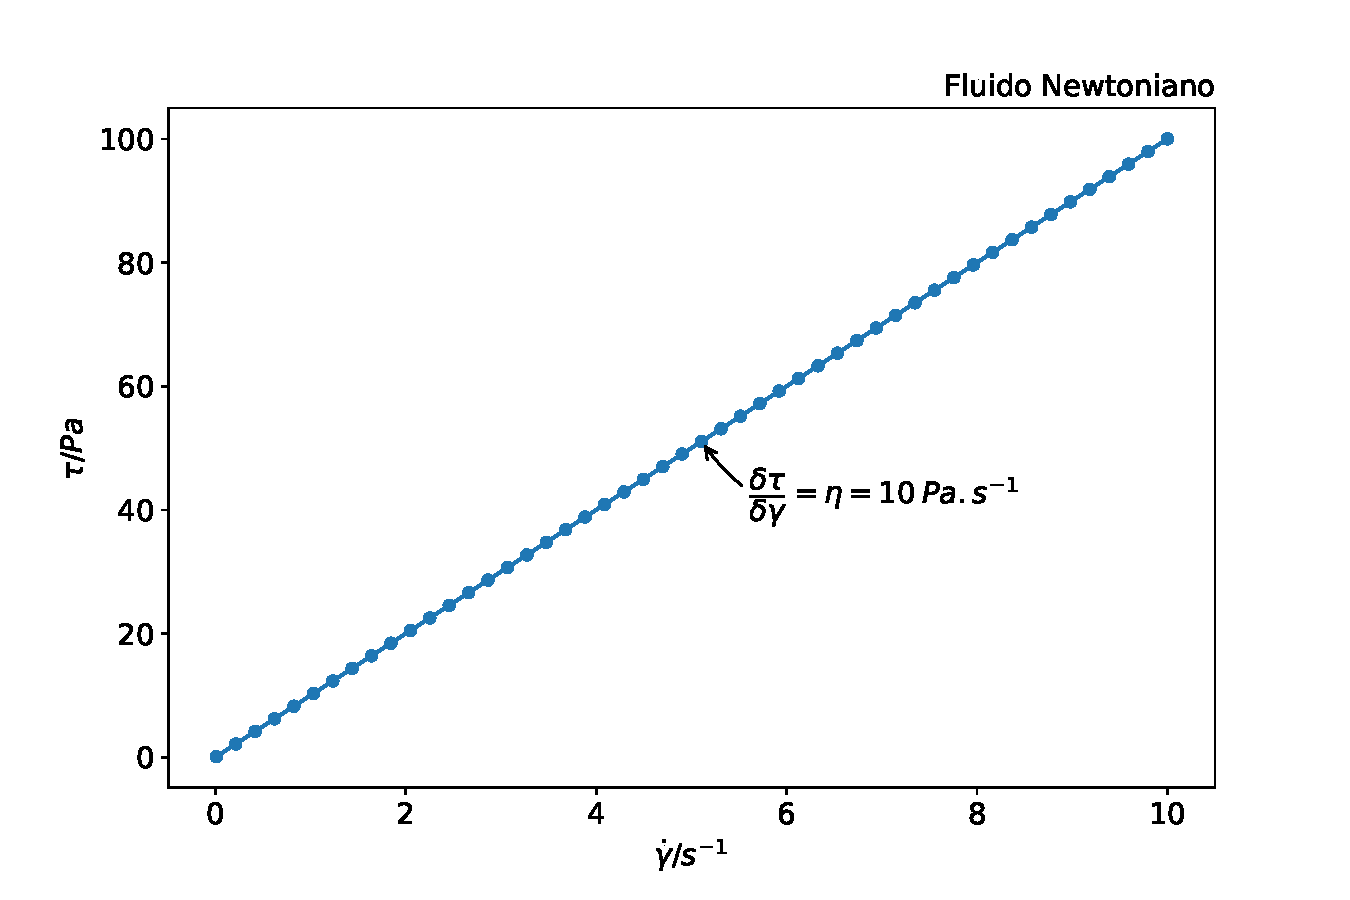
\includegraphics[width=\textwidth]{./imagens/reologia/newtoniano_exemplo_tauGP}
					\caption{\(\tau \times \dot{\gamma}\)}
					\label{fig:reol_newt_tauGP}
				\end{subfigure}%
				\begin{subfigure}[t]{.5\textwidth}
					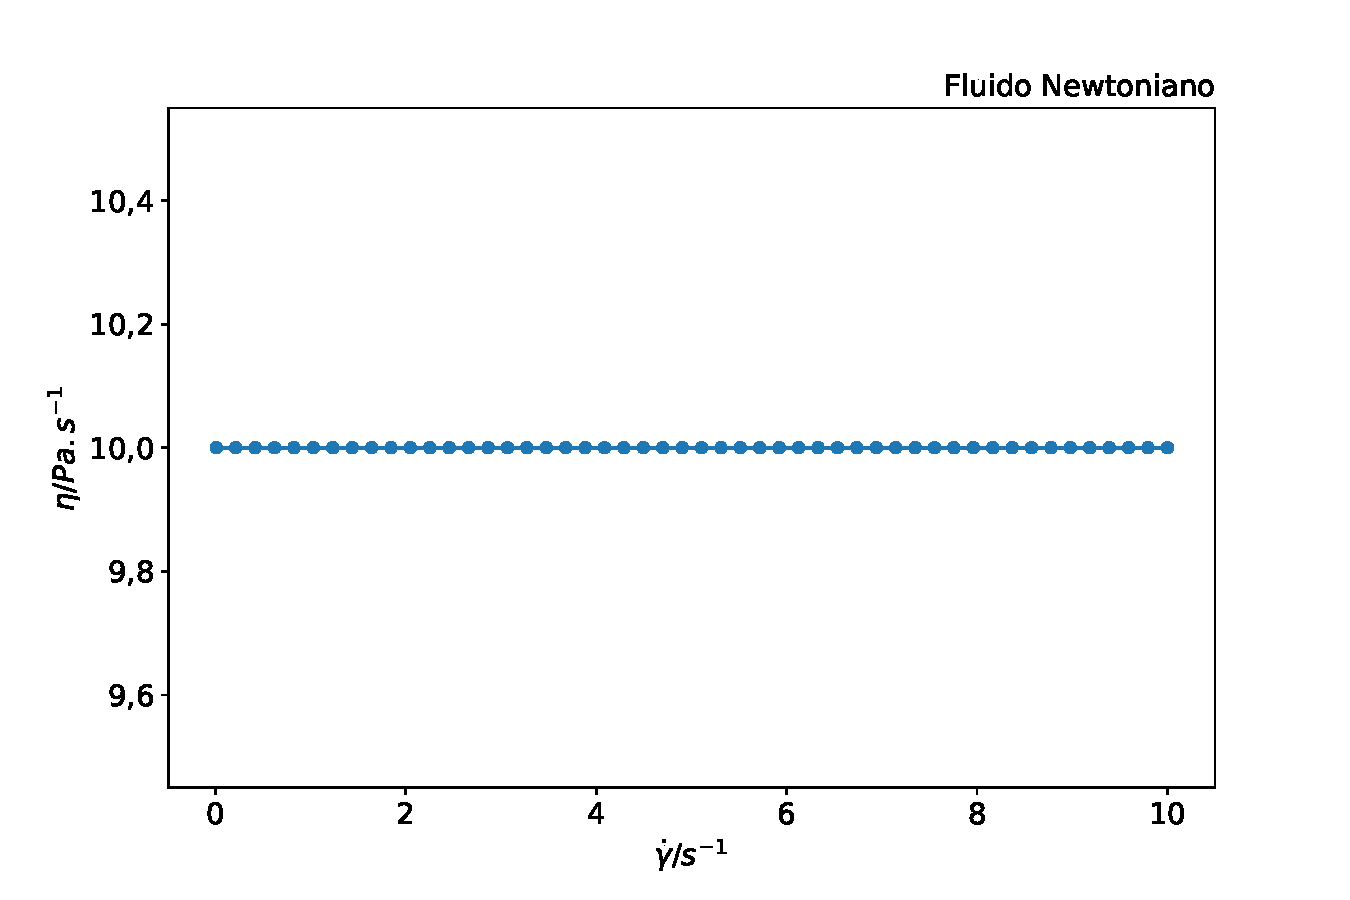
\includegraphics[width=\textwidth]{./imagens/reologia/newtoniano_exemplo_etaGP}
					\caption{\(\eta \times \dot{\gamma}\)}
					\label{fig:reol_newt_etaGP}
				\end{subfigure}
				\caption{Exemplos de curvas de fluxo. (\ref{fig:reol_newt_tauGP}) Método para obtenção da viscosidade. (\ref{fig:reol_newt_etaGP}) Dependência da viscosidade com a taxa de cisalhamento, mostrando que o valor é constante.}
				\label{fig:reol_newt_exemplos}
			\end{figure}
				
			\subsection{Sólidos Hookeanos}
			
			Sólidos hookeanos possuem uma constante elástica \(G\) que relaciona a tensão \(\tau\) aplicada e a deformação \(\gamma\) (Eq. \ref{eqn:Hooke}).
			
			\begin{equation}
				\tau = G\gamma
				\label{eqn:Hooke}
			\end{equation}
			
			A deformação de um sólido Hookeano pode ser tanto compressiva quando extensiva, dependendo do sinal de \(\gamma\), e consequentemente a tensão retornada possui a direção oposta da tensão aplicada inicialmente. 
			
			O modelo físico associado ao sólido Hookeano é a mola. É possível que uma mola, quando estendida demasiadamente, não retorne à sua extensão original. Isso ocorre porque a Eq. \ref{eqn:Hooke} se aplica somente a uma região dos possíveis valores de \(\gamma\). A fig X mostra o comportamento Hookeano de amostras.
			
			% todo: colocar uma figura do Goodwin e Hughes de viscosidade, para mostrar o comportamento não Hookeano.
			
			\subsection{Fluidos não-Newtonianos}
			
			Fluidos que não obedecem a lei de Newton (Eq. \ref{eqn:Newton}), portanto possuem valores de viscosidade dependentes da taxa de cisalhamento, são chamados de fluidos não-Newtonianos. Dentro dessa classificação, há vários tipos de fluido, dependendo de como \(\eta\) varia com (\(\dot{\gamma}\)). Alguns dos tipos possíveis são:
			
			\begin{itemize}[noitemsep]
				\item Plásticos: Viscosidade inicial é muito alta ou, teoricamente, infinita, até a tensão atingir um valor específico, chamado de tensão limite ou \emph{yield-stress}, quando o material começa a fluir. Exemplo: Manteiga, géis. % todo: achar se o termo é tensão limite mesmo
				\item Pseudoplásticos ou \emph{shear-thinning}: Viscosidade alta, mas finita, em baixas taxas de cisalhamento, e decai com o aumento da taxa de cisalhamento, atingindo um valor mínimo. Exemplo: soluções de micelas gigantes.
				\item Dilatantes: Viscosidade baixa a baixas taxas de cisalhamento, e aumenta com o aumento da taxa. Exemplo: Dispersões de amido em água.
			\end{itemize}
			
			% Todo: colocar a figura dos vários tipos de comportamento aqui.
			
			% todo: pensar melhor sobre isso de contribuições elásticas e viscosas. O que eu escrevi aqui é o oposto do que aparece no diagrama de frequência, com a viscosidade complexa. Qual é a relação?
			
			Sob taxas de cisalhamento baixas, micelas gigantes em solução estão emaranhadas. Isso dificulta a movimentação do solvente e da solução como um todo, resultado em uma viscosidade aparente alta. Nesse regime, o comportamento elástico predomina. Quanto maior for o entrelaçamento das micelas, maior é a contribuição do comportamento elástico, e maior é a viscosidade aparente. À medida que a taxa é aumentada, as micelas gigantes começam a se alinhar ao fluxo, de modo a diminuir o gradiente de velocidade que cada cadeia sente. Isso facilita o fluxo e diminui a estruturação que resulta no comportamento elástico, o que acaba diminuindo a viscosidade aparente.
			
			Após um valor específico de taxa de cisalhamento, a viscosidade atinja um mínimo pois não há mais como aumentar o alinhamento das micelas. Nessa situação, a viscosidade aparente é predominantemente devido ao solvente, e a contribuição Newtoniana é predominante. A figura \ref{fig:reol_pseudoplastico_exemplos} mostra a curva de fluxo de um material pseudoplástico, tanto .\footnote{Construção: vide apêndice \ref{sec:apn_tratamento_CF}. Parâmetros: Modelo de Carreau, \(\eta_0=10\), \(\eta_{\infty}=1\), \(\dot{\gamma}_b=10\), \(n=10\).} É possível que as cadeias comecem a se estruturar, formando \emph{shear induced structures}, mas isso não foi observado neste trabalho.
	
			\begin{figure}[H]
				\begin{subfigure}[t]{.5\textwidth}
					\includegraphics[width=\textwidth]{./imagens/reologia/pseudoplastico_tau}
					\caption{\(\tau \times \dot{\gamma}\)}
					\label{fig:reol_pseudo_tauGP}
				\end{subfigure}%
				\begin{subfigure}[t]{.5\textwidth}
					\includegraphics[width=\textwidth]{./imagens/reologia/pseudoplastico_eta}
					\caption{\(\eta \times \dot{\gamma}\)}
					\label{fig:reol_pseudo_etaGP}
				\end{subfigure}
				\caption{Exemplos de curvas de fluxo de um fluido pseudoplástico. (\ref{fig:reol_newt_tauGP}) Tensão aplicada em função da taxa de cisalhamento. (\ref{fig:reol_newt_etaGP}) Derivada de (\ref{fig:reol_newt_tauGP}) em função da taxa de cisalhamento.}
				\label{fig:reol_pseudoplastico_exemplos}
			\end{figure}
			
			No entanto, as curvas de fluxo são frequentemente plotadas na escala log-log. Nesse tipo de gráfico (Fig. \ref{fig:reol_pseudoplastico_loglog}), é possível observar a região com viscosidade constante em baixas taxas de cisalhamento, chamada de platô Newtoniano, devido à sua constância. Essa valor também é chamado de viscosidade no repouso, \(\eta_0\).
			
			\begin{figure}[H]
				\centering
				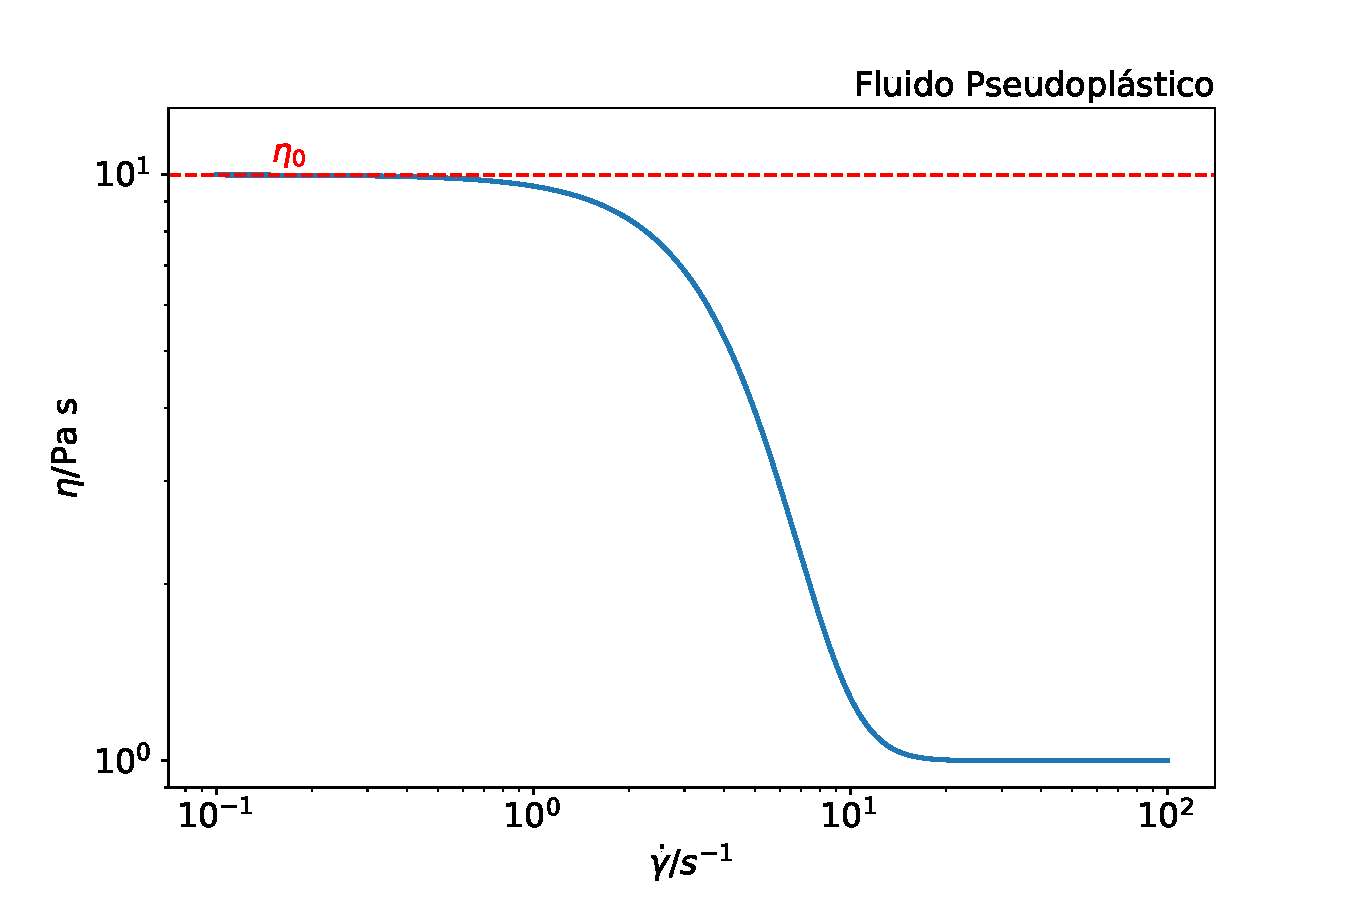
\includegraphics[width=0.7\textwidth]{./imagens/reologia/Pseudoplastico_loglog}
				\caption{Curva de fluxo de um fluído pseudoplástico na escala log-log, mostrando o valor da viscosidade no repouso, \(\eta_0\).}
				\label{fig:reol_pseudoplastico_loglog}
			\end{figure}
		
			Para obter o valor da viscosidade no repouso, é possível tanto realizar um ajuste linear da região inicial na escala log-log, ou ajustar um modelo à curva, como o modelo de Cross, Carreau e Carreau-Yasuda. Mais informações sobre a modelagem estão no apêndice \ref{sec:apn_tratamento_CF}.

		\section{Reologia oscilatória}
			\subsection{Princípios e aquisição de dados}
			
			As análises oscilatórias podem ser utilizadas para obter informações reológicas mais completas sobre um material. Variando-se a frequência de perturbação, é possível obter o espectro mecânico do material, onde se observa as contribuições elástica e viscosa em função da frequência de perturbação mecânica.
			
			Ao material, é aplicada uma deformação \(\gamma\) que varia com o tempo de acordo com a Eq. \ref{eqn:osc_gamma_t}.
			
			\begin{equation}
				\gamma(t)=\gamma_0\cos(\omega t)
				\label{eqn:osc_gamma_t}
			\end{equation}
			
			\noindent onde \(\gamma_0\) é a deformação máxima e \(\omega\) é a frequência de perturbação. As deformações aplicadas ao material devem ser tais que não ocorra desestruturação do mesmo. Por exemplo, uma deformação muito grande pode causar a quebra de ligações químicas de um polímero, o que altera irreversivelmente as suas características reológicas. Por esse motivo, é necessário modular também a tensão aplicada.
			
			Um material elástico responde à deformação imediatamente com uma força no sentido oposto ao sentido da deformação. Já materiais viscosos respondem à deformação quando há uma mudança na direção, ou seja, a resposta desses materiais é totalmente defasada em relação à aplicação da deformação. Já materiais viscoelásticos, por terem componentes de ambos os tipos, possuem uma defasagem intermediária. O grau dessa defasagem é proporcional ao grau de comportamento elástico e viscoso. Levando isso em consideração, a tensão \(\tau\)  é expressa de acordo com a Eq. \ref{eqn:osc_tau_t}.
			
			\begin{equation}
				\tau = \tau_0\cos(\omega t - \theta)
				\label{eqn:osc_tau_t}
			\end{equation}
			
			\noindent onde \(\tau_0\) é a tensão máxima (determinada no experimento oscilatório de amplitude) e \(\theta\) é o ângulo de defasagem.
			
			As expressões \ref{eqn:osc_gamma_t} e \ref{eqn:osc_tau_t} podem ser reescritas utilizando a relação de Euler, Eq. \ref{eqn:Euler}, resultando nas expressões \ref{eqn:osc_gamma_im} e \ref{eqn:osc_tau_im}, onde utilizou-se um acento circunflexo para diferenciar as expressões. Essa transformação facilita a manipulação matemática.
			
			\begin{equation}
				e^{ix} = \cos(x) + i\sin(x)
				\label{eqn:Euler}
			\end{equation}
			
			\begin{equation}
				\hat{\gamma} = \gamma_0 e^{i\omega t}
				\label{eqn:osc_gamma_im}
			\end{equation}
			
			\begin{equation}
				\hat{\tau} = \tau_0 e^{i(\omega t - \theta)}
				\label{eqn:osc_tau_im}
			\end{equation}
			
			A partir dessas relações, é possível utilizar a equação de Hooke (Eq. \ref{eqn:Hooke}) para encontrar o módulo elástico do material, na notação imaginária, \(\hat{G}\) (Eq. \ref{eqn:osc_transform_G}).
			
			\begin{equation}
				\hat{\tau} = \hat{G}\hat{\gamma} \to \hat{G} = \dfrac{\hat{\tau}}{\hat{\gamma}}    \to 
				\hat{G} = \dfrac{\tau_0}{\gamma_0} \dfrac{e^{i(\omega t - \theta)}}{e^{i\omega t}} \to
				\hat{G} = \dfrac{\tau_0}{\gamma_0} e^{-i\theta}
				\label{eqn:osc_transform_G}
			\end{equation}
			
			Utilizando-se a equação de Euler novamente, mas voltando para o domínio dos senos e cossenos, obtemos a Eq. \ref{eqn:osc_volta_senos_G}:
			
			\begin{equation}
				\hat{G} = \dfrac{\tau_0}{\gamma_0} \left( \cos(\theta) + i\sin(\theta) \right)
				\label{eqn:osc_volta_senos_G}
			\end{equation}
			
			Nessa equação, o módulo total \(\hat{G}\) foi dividido em dois termos, um em fase à deformação \(\cos(\theta)\) e outro 90° fora de fase, \(\sin(\theta)\). Esses dois termos são diretamente relacionáveis às componentes elástica e viscosa de um material. Dessa maneira, é possível separar o módulo total complexo \(\hat{G}\) em dois módulos (Eq. \ref{eqn:osc_G_complexo}), o módulo elástico, G' (Eq. \ref{eqn:osc_g1linha}), e o módulo viscoso, G'' (Eq. \ref{eqn:osc_g2linha}).
			
			\begin{equation}
				\hat{G} = G' + iG''
				\label{eqn:osc_G_complexo}
			\end{equation}
			
			\begin{equation}
				G' = \dfrac{\tau_0}{\gamma_0} \cos(\theta)
				\label{eqn:osc_g1linha}
			\end{equation}
			
			\begin{equation}
				G'' = \dfrac{\tau_0}{\gamma_0} \sin(\theta)
				\label{eqn:osc_g2linha}
			\end{equation}
			
			Portanto, para conseguir separar os valores dos módulos G' e G'', o reômetro necessita medir o módulo total e o ângulo de defasagem, sendo possível assim separar os componentes. Vale notar que a tangente do ângulo de defasagem é a relação \(G''/G'\) (Eq. \ref{eqn:osc_tan_teta})
			
			\begin{equation}
				\tan(\theta) = \dfrac{\sin(\theta)}{\cos(\theta)} = \dfrac{G''}{G'}
				\label{eqn:osc_tan_teta}
			\end{equation}
			
			A Figura \ref{fig:osc_simulacoes} mostra uma série de simulações do modelo apresentado aqui. A deformação em função do tempo foi calculada, e o ângulo de defasagem foi aumentado gradativamente de 0° para 90°. 
			% todo: descobrir e colocar os ângulos aqui
			
			\begin{figure}[H]
				\begin{subfigure}[t]{0.3\textwidth}
					\centering
					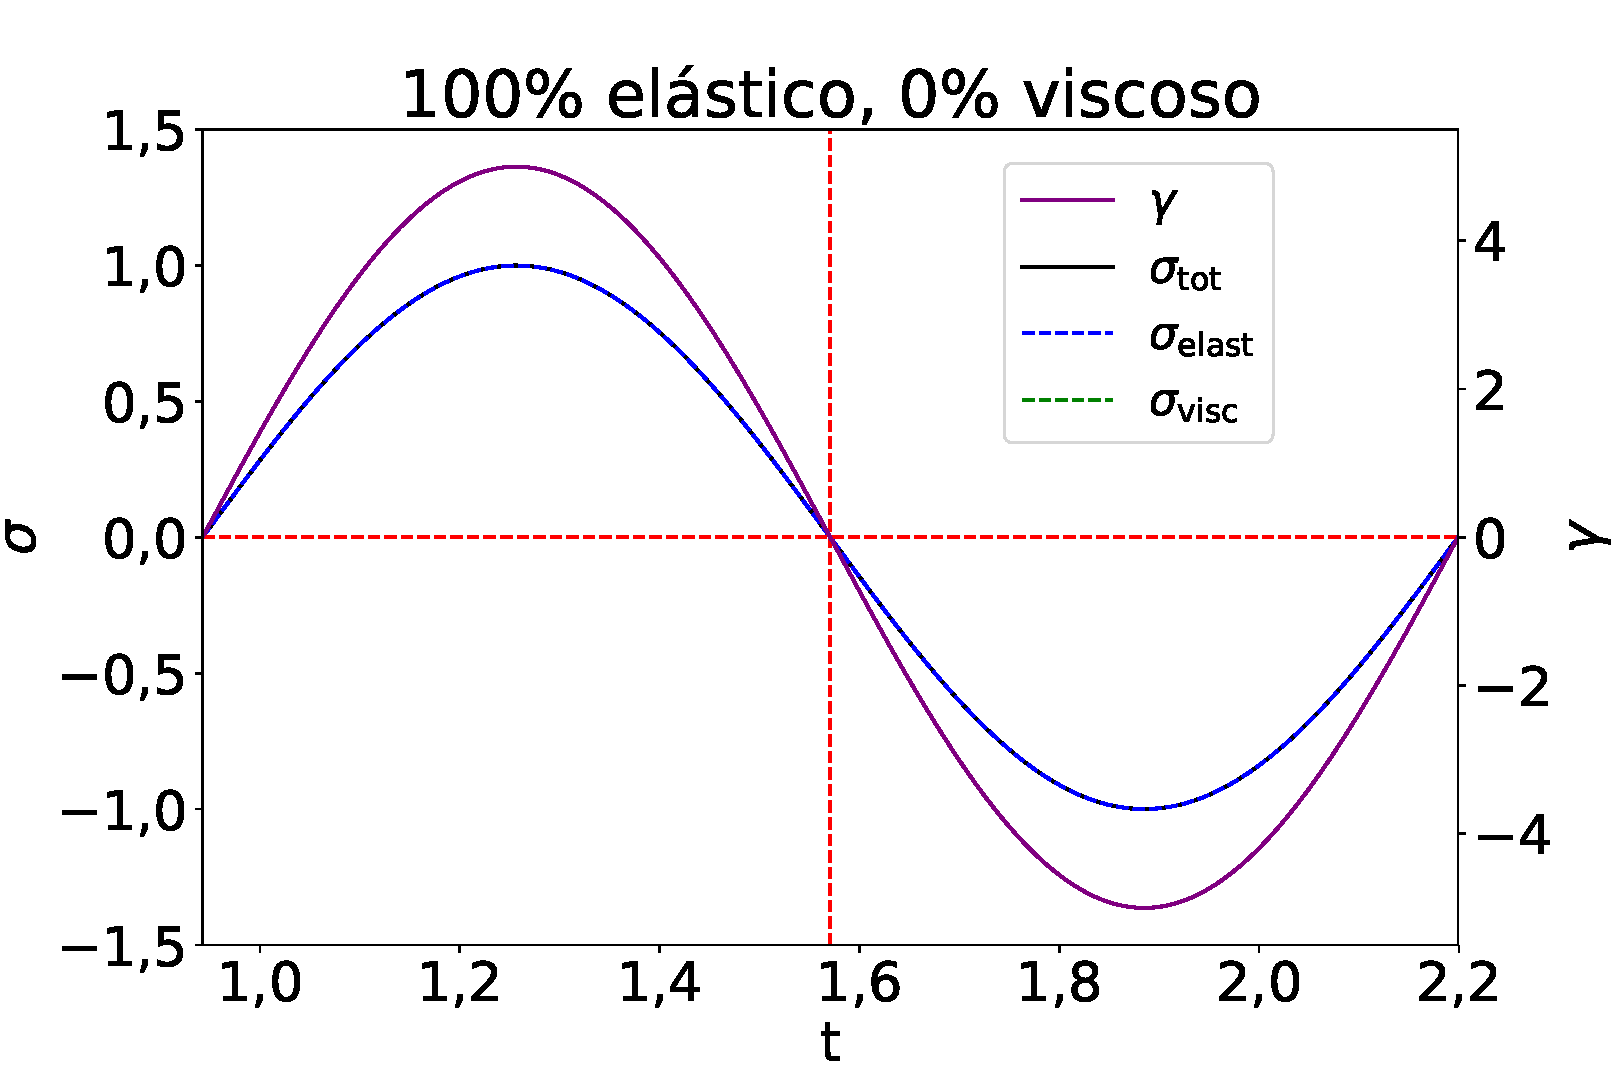
\includegraphics[width=\textwidth]{./imagens/reologia/Simulacao_visc_0}
					\caption{\(\theta=0°\)}
					\label{fig:osc_sim0}
				\end{subfigure}%
				\begin{subfigure}[t]{0.3\textwidth}
					\centering
					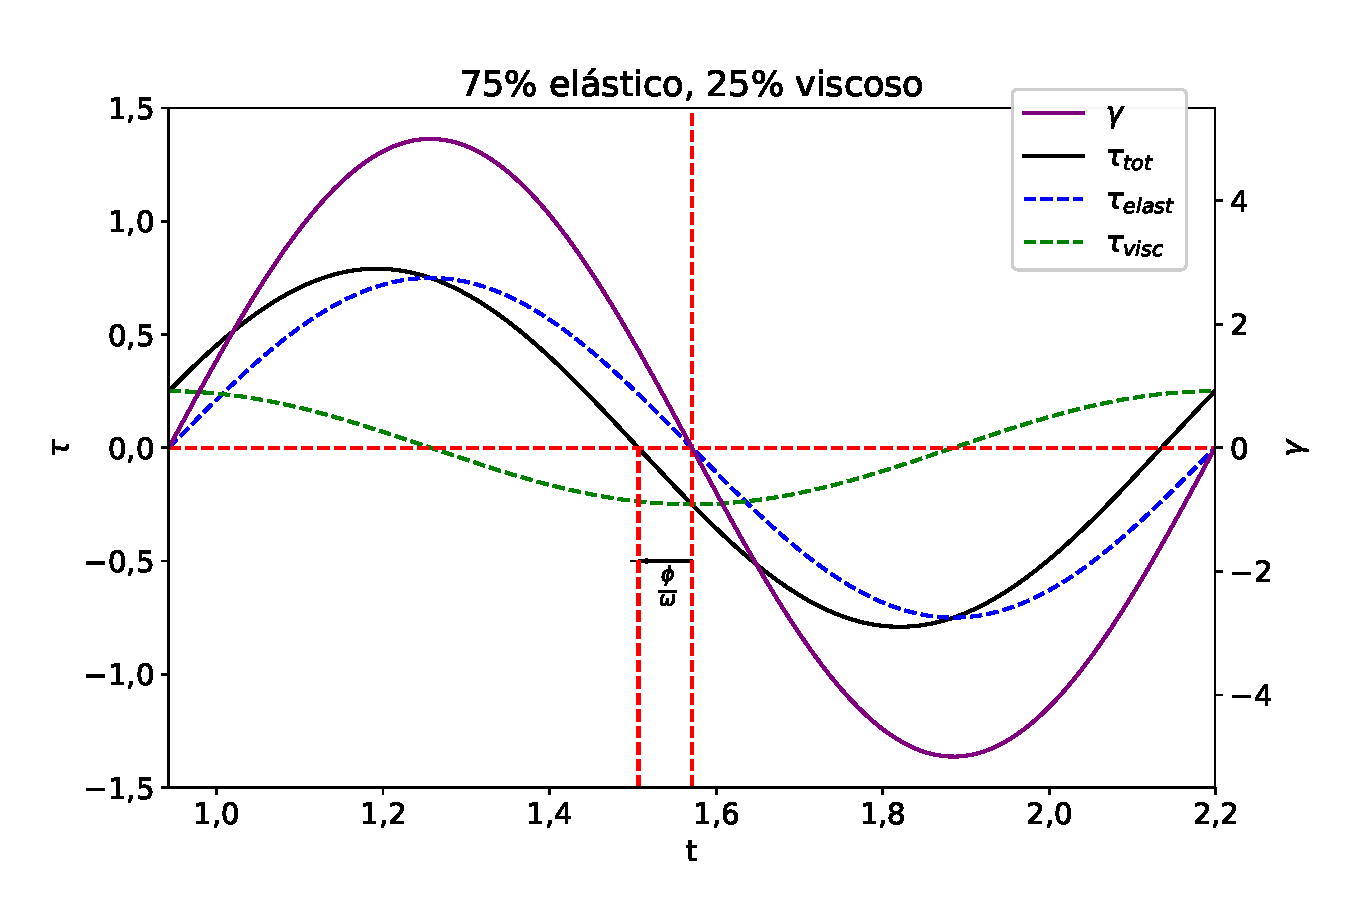
\includegraphics[width=\textwidth]{./imagens/reologia/Simulacao_visc_25}
					\caption{\(\theta=18°\)}
					\label{fig:osc_sim25}
				\end{subfigure}%
				\begin{subfigure}[t]{0.3\textwidth}
					\centering
					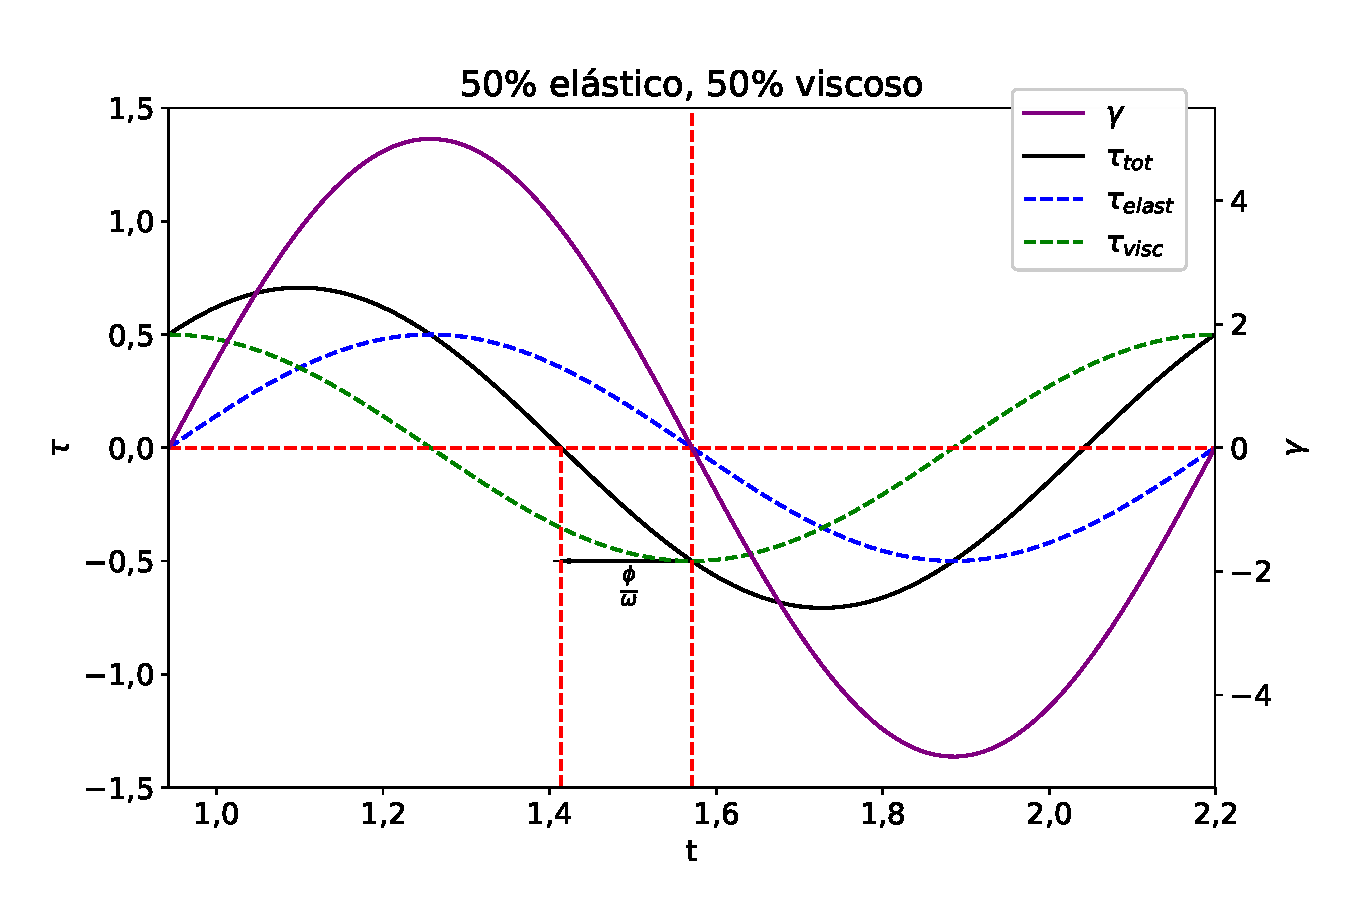
\includegraphics[width=\textwidth]{./imagens/reologia/Simulacao_visc_50}
					\caption{\(\theta=45°\)}
					\label{fig:osc_sim50}
				\end{subfigure}
			
				\begin{subfigure}[t]{0.3\textwidth}
					\centering
					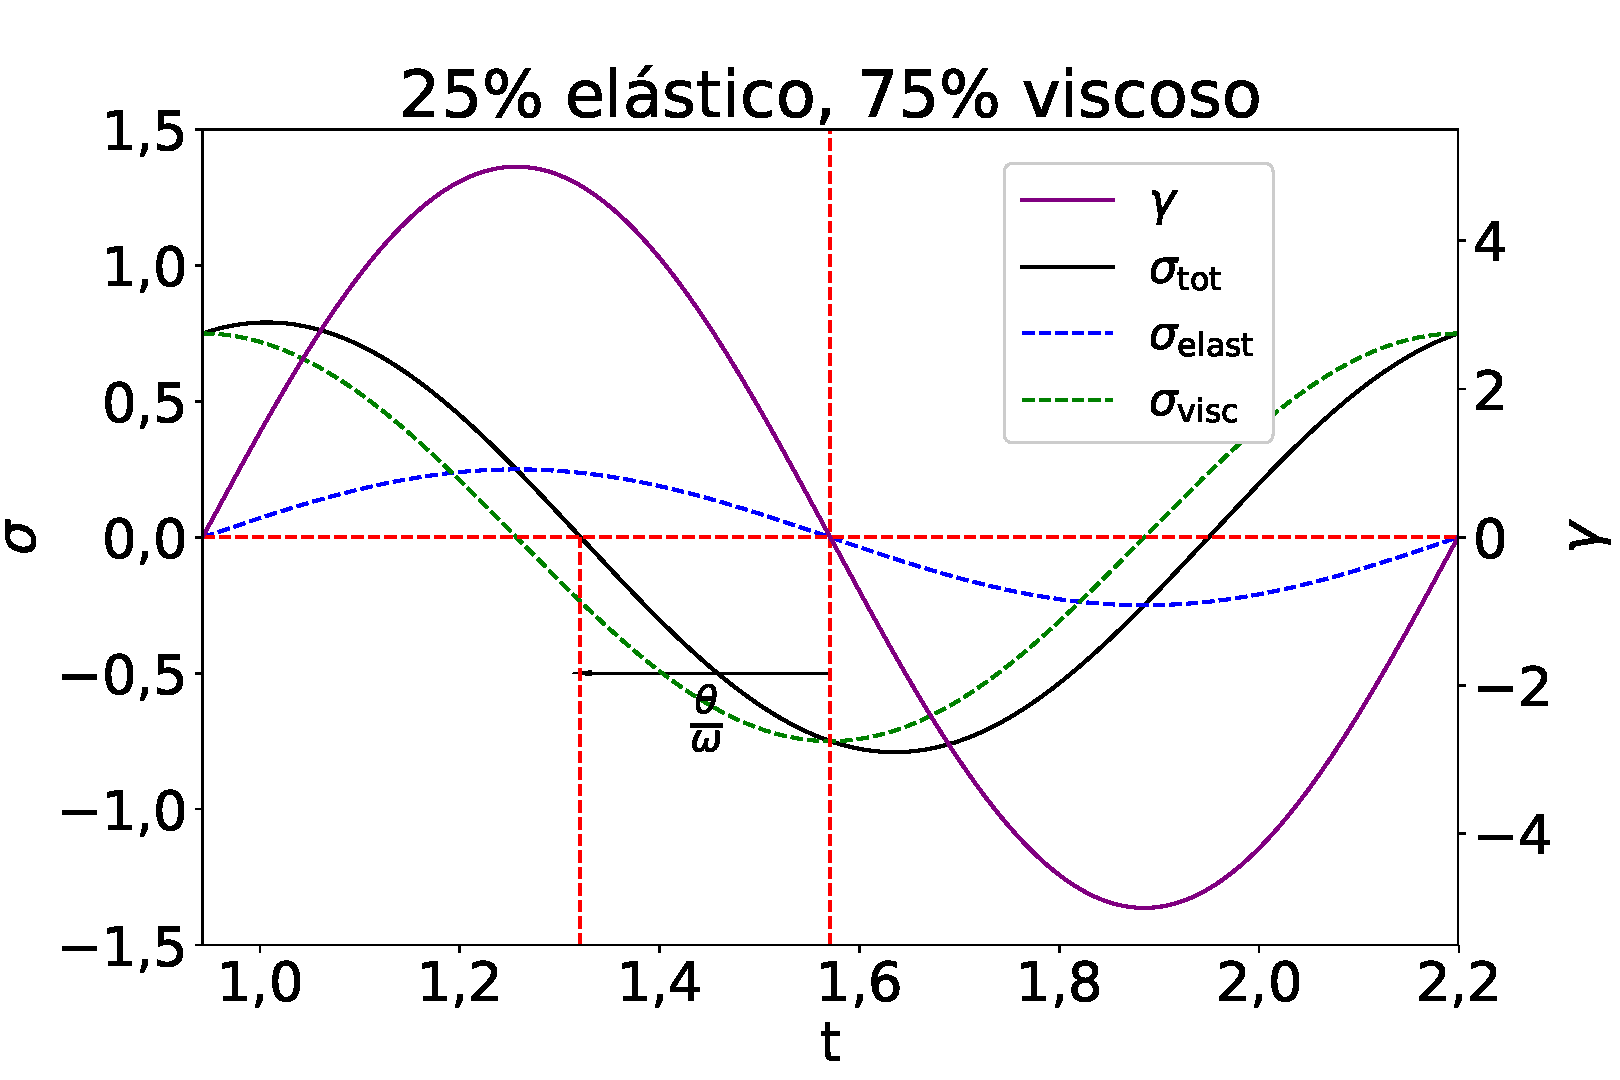
\includegraphics[width=\textwidth]{./imagens/reologia/Simulacao_visc_75}
					\caption{\(\theta=72°\)}
					\label{fig:osc_sim75}
				\end{subfigure}%
				\begin{subfigure}[t]{0.3\textwidth}
					\centering
					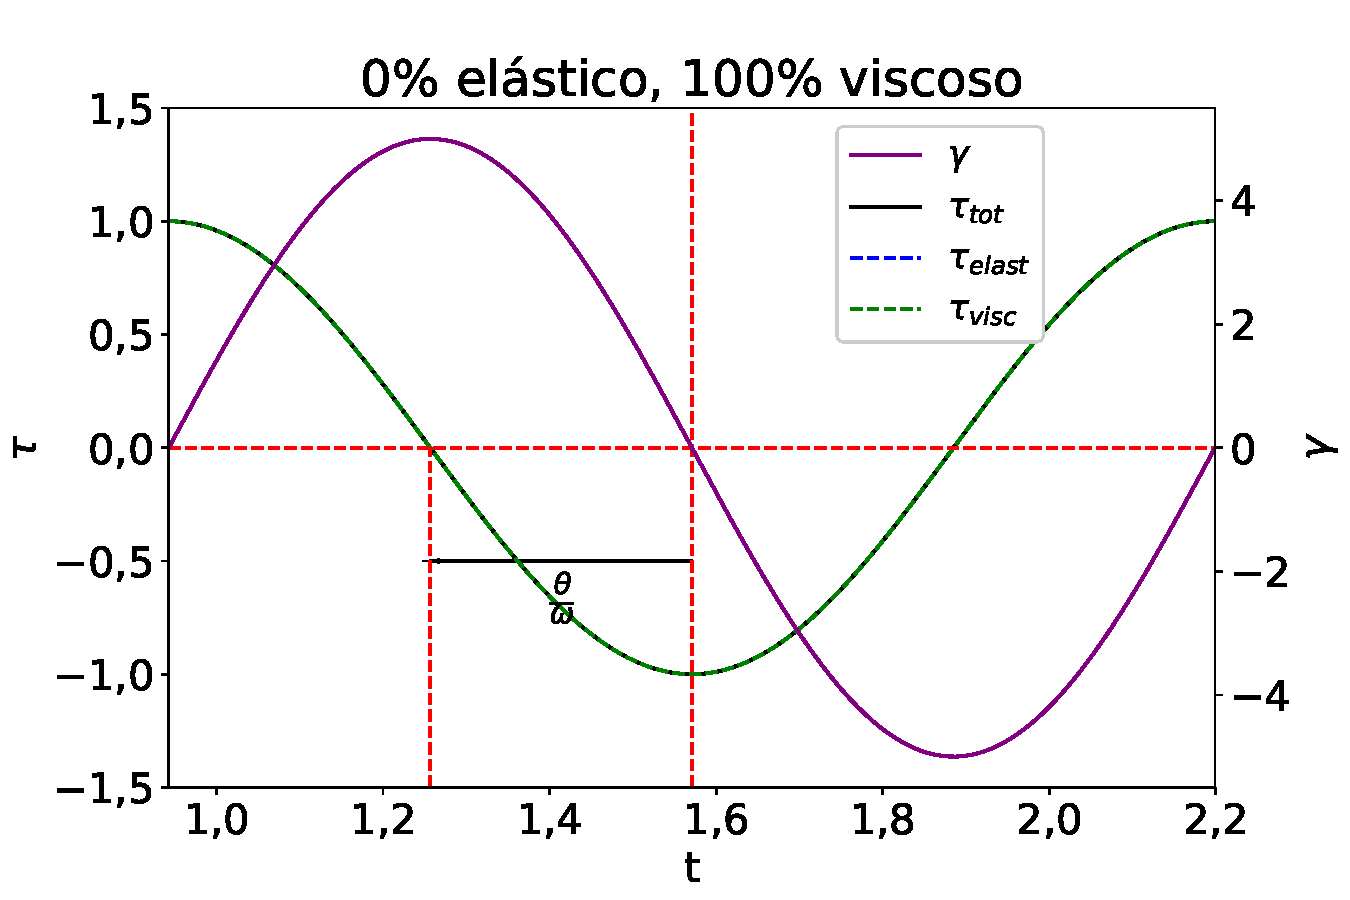
\includegraphics[width=\textwidth]{./imagens/reologia/Simulacao_visc_100}
					\caption{\(\theta=90°\)}
					\label{fig:osc_sim100}
				\end{subfigure}%
%				\begin{subfigure}[t]{0.3\textwidth}
%					\centering
%					\includegraphics[width=\textwidth]{}
%					\label{fig:}
%				\end{subfigure}
			\caption{Simulações do comportamento de um fluido sob cisalhamento cossenoidal. As imagens mostram a deformação \(\gamma\) em função do tempo, a tensão total \(\tau\) de resposta em função do tempo, decomposta em suas componentes elástica e viscosa. No título de cada gráfico está a contribuição, em porcentagem, de cada componente do material. O ângulo de defasagem está ilustrado na figura.}
			\label{fig:osc_simulacoes}
			\end{figure}  % todo: colocar o código para essa figura nos apêndices
			
			\subsection{Modelo de Maxwell}
			
			O modelo de Maxwell é construído juntando-se um elemento elástico (mola) e um elemento viscoso (dissipador), ideais, em série. A Figura \ref{fig:ilust_modelo_maxwell} ilustra essa construção.
			
			\begin{figure}[H]
				\centering
				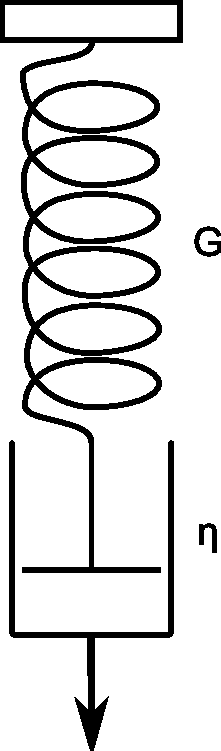
\includegraphics[width=1.5cm]{./imagens/reologia/maxwell_mola_dissipador}
				\caption{Modelo de Maxwell: Mola com constante elástica \(G\) e dissipador com constante viscosa \(\eta\) em série}
				\label{fig:ilust_modelo_maxwell}
			\end{figure}

			 É possível expressar a taxa de cisalhamento do modelo de Maxwell como a soma das taxas de cisalhamento dos elementos individuais (Eq. \ref{eqn:Maxwell_soma}). 
			 
			\begin{equation}
				\dot{\gamma}_{\textrm{total}} =  \dot{\gamma}_{\textrm{viscoso}} + \dot{\gamma}_{\textrm{elástico}} \to
				\dfrac{\mathrm{d}\gamma}{\mathrm{d}t} = \dfrac{1}{\eta}\tau + \dfrac{1}{G}\dfrac{\mathrm{d}\tau}{\mathrm{d}t}
				\label{eqn:Maxwell_soma}
			\end{equation}
			
			Para uma deformação constante, \(\frac{\mathrm{d}\gamma}{\mathrm{d}t}=0\), a Eq. \ref{eqn:Maxwell_soma} se torna uma equação diferencial (Eq. \ref{eqn:Maxwell_diferencial}).
			
			\begin{equation}
				\dfrac{1}{\eta}\tau + \dfrac{1}{G}\dfrac{d\tau}{dt} = 0
				\label{eqn:Maxwell_diferencial}
			\end{equation}
			
			Utilizando as condições de contorno necessárias, essa equação pode ser resolvida, resultando em (Eq. \ref{eqn:Maxwell_dif_resolvida}):
			
			\begin{equation}
				\tau(t) = \tau_0 e^{\left( -\frac{G}{\eta}t \right)}
				\label{eqn:Maxwell_dif_resolvida}
			\end{equation}
			
			O termo exponencial na Eq. \ref{eqn:Maxwell_dif_resolvida} possui unidade de tempo e é a relação entre as componentes elástica e viscosa do material. Essa relação recebe o nome de tempo de relaxação, \(\tau_{\textrm{rel}}\) (Eq. \ref{eqn:Maxwell_tempo_rel_def})
			
			\begin{equation}
				\tau(t) = \tau_0 e^{\sfrac{-t}{\tau_{\textrm{rel}}}}
				\label{eqn:Maxwell_tempo_rel_def}
			\end{equation}
		
			O tempo de relaxação é o tempo em que a tensão inicial demora para cair ao valor de \(\sfrac{1}{e}\) do valor inicial. É interessante notar que em tempos pequenos, relativos a \(\tau_{\textrm{rel}}\), o material responde com a tensão inicial total. Essa é a resposta imediata da mola. Porém, com o tempo, à medida que \(t\to\tau_{\textrm{rel}}\), a tensão começa a decair exponencialmente e depois, em \(t \gg \tau_{\textrm{rel}}\), tende a zero. Nessa situação, o dissipador difundiu toda a energia inicial aplicada.
			
			A expressão \ref{eqn:Maxwell_soma} pode ser rearranjada utilizando o tempo de relaxação (\ref{eqn:Maxwell_tempo_rel_def}).
			
			\begin{equation}
				\dfrac{\mathrm{d}\gamma}{\mathrm{d}t} = \dfrac{1}{\eta}\tau + \dfrac{1}{G}\dfrac{\mathrm{d}\tau}{\mathrm{d}t} \to 
				\tau = -\dfrac{\eta}{G} \dfrac{\mathrm{d}\tau}{\mathrm{d}t} + \eta\dfrac{\mathrm{d}\gamma}{\mathrm{d}t} =
				-\tau_{\textrm{rel}} \dfrac{\mathrm{d}\tau}{\mathrm{d}t} + \eta\dfrac{\mathrm{d}\gamma}{\mathrm{d}t}
				\label{eqn:Maxwell_inicio_g1g2}
			\end{equation}
			
			É possível substituir as expressões de tensão e \ref{eqn:osc_gamma_im} e \ref{eqn:osc_tau_im} na expressão \ref{eqn:Maxwell_inicio_g1g2} para obter uma expressão em função do tempo, da frequência e do ângulo de fase. Já realizando as derivações, obtemos:
			
			\begin{equation}
				\tau_0 e^{i \left( \omega t - \theta \right)} = - \tau_{\textrm{rel}} \tau_0 i\omega e^{i \left( \omega t - \theta \right)}     +       \eta i\omega\gamma_0e^{i\omega t}
				\label{eqn:Maxwell_substituicao}
			\end{equation}
			
			Em comum a todos os termos é a constante \(e^{i\omega t}\). Dividindo ambos os lados por essa constante, agrupando os termos com \(e^{-i\theta}\) e substituindo a viscosidade por \(G\tau_{\textrm{rel}}\), temos:
			
			\begin{equation}
				\tau_0e^{-i\theta} \left(   1 + i\omega\tau_{\textrm{rel}}  \right) = i\omega G\tau_{\textrm{rel}}\gamma_0 \to
				\tau_0e^{-i\theta} = \dfrac{i\omega G\tau_{\textrm{rel}}\gamma_0}{\left(   1 + i\omega\tau_{\textrm{rel}}  \right)}
				\label{eqn:Maxwell_intermediario}
			\end{equation}
			
			O termo à esquerda da Eq. \ref{eqn:Maxwell_intermediario} é similar à definição do módulo elástico complexo, Eq. \ref{eqn:osc_transform_G}, sendo necessário somente dividir ambos os lados por \(\gamma_0\). Realizando a substituição, temos:
			
			\begin{equation}
				\hat{G} = \dfrac{\tau_0e^{-i\theta}}{\gamma_0} = \dfrac{i\omega G\tau_{\textrm{rel}}}{\left(   1 + i\omega\tau_{\textrm{rel}}  \right)}
				\label{eqn:Maxwell_complexo_antes_sep}
			\end{equation}
			
			Seguindo o princípio de que o módulo complexo \(\hat{G}\) pode ser dividido em uma parte imaginária e uma parte real, podemos realizar o mesmo com a Eq. \ref{eqn:Maxwell_complexo_antes_sep} multiplicando-se a fração por \(\frac{\left(   1 - i\omega\tau_{\textrm{rel}}  \right)}{\left(   1 - i\omega\tau_{\textrm{rel}}  \right)}\).
			
			\begin{equation}
				\hat{G} = \dfrac{  i\omega G\tau_{\textrm{rel}} - i^2 \omega^2 G \tau_{\textrm{rel}}^2        }{  1 - i^2\omega^2 \tau_{\textrm{rel}}^2          }
				\label{eqn:Maxwell_complexo_antes_sep2}
			\end{equation}
			
			Separando as partes imaginárias das partes reais e substituindo \(i^2 = -1\):
			
			\begin{equation}
				\hat{G} = \dfrac{   \omega^2 G \tau_{\textrm{rel}}^2       }{  1 + \omega^2 \tau_{\textrm{rel}}^2      } + i \dfrac{   \omega G \tau_{\textrm{rel}}        }{ 1 + \omega^2 \tau_{\textrm{rel}}^2 }
				\label{eqn:Maxwell_substituido}
			\end{equation}
			
			Seguindo a expressão \ref{eqn:osc_G_complexo}, \(\hat{G} = G' + iG''\), podemos definir o módulo elástico de acordo com o modelo de Maxwell como:
			
			\begin{equation}
				G' = \dfrac{ G \omega^2 \tau_{\textrm{rel}}^2   }{  1 + \omega^2 \tau_{\textrm{rel}}^2      }
				\label{eqn:Maxwell_G1_def}
			\end{equation}
			
			E o módulo viscoso, G'', como:
			
			\begin{equation}
				G'' = \dfrac{  G \omega  \tau_{\textrm{rel}}        }{ 1 + \omega^2 \tau_{\textrm{rel}}^2 }
				\label{eqn:Maxwell_G2_def}
			\end{equation}
			
			É interessante notar que a relação \(\sfrac{G''}{G'}\), que equivale a \(\tan(\theta)\) (\ref{eqn:osc_tan_teta}), também se relaciona com o tempo de relaxação:
			
			\begin{equation}
				\tan(\theta) = \dfrac{G''}{G'} = \dfrac{1}{\omega\tau_{\textrm{rel}}}
				\label{eqn:Maxwell_cruzamento}
			\end{equation}
			
			Com isso, é possível determinar o tempo de relaxação de um fluido Maxwelliano através da frequência do ponto de cruzamento de G' e G''. Lembrando que \(\omega\) é a frequência de perturbação, e o inverso da frequência é o tempo de observação, podemos relacionar essa relação com o número de Deborah, Eq. \ref{eqn:Deborah}.
			
			\begin{equation}
				\dfrac{1}{\omega\tau_{\textrm{rel}}} = \dfrac{ t_{\textrm{observação}  }}{ \tau_{\textrm{rel}}  } = \dfrac{1}{D_e}
				\label{eqn:Maxwell_cruzamento_Deborah}
			\end{equation}

			A reologia oscilatória geralmente é expressa em termos de G' e G'' em função da frequência, na escala logarítmica. A Fig. \ref{fig:modelo_maxwell} mostra duas curvas simuladas para um material com tempo de relaxação de 10 s.$rad^{-1}$ e um módulo \(G\) de 10 Pa. Nessa figura estão mostrado como se obtêm visualmente os parâmetros \(G\) e \(\tau_{\textrm{rel}}\).
			
			\begin{figure}[H]
				\centering
				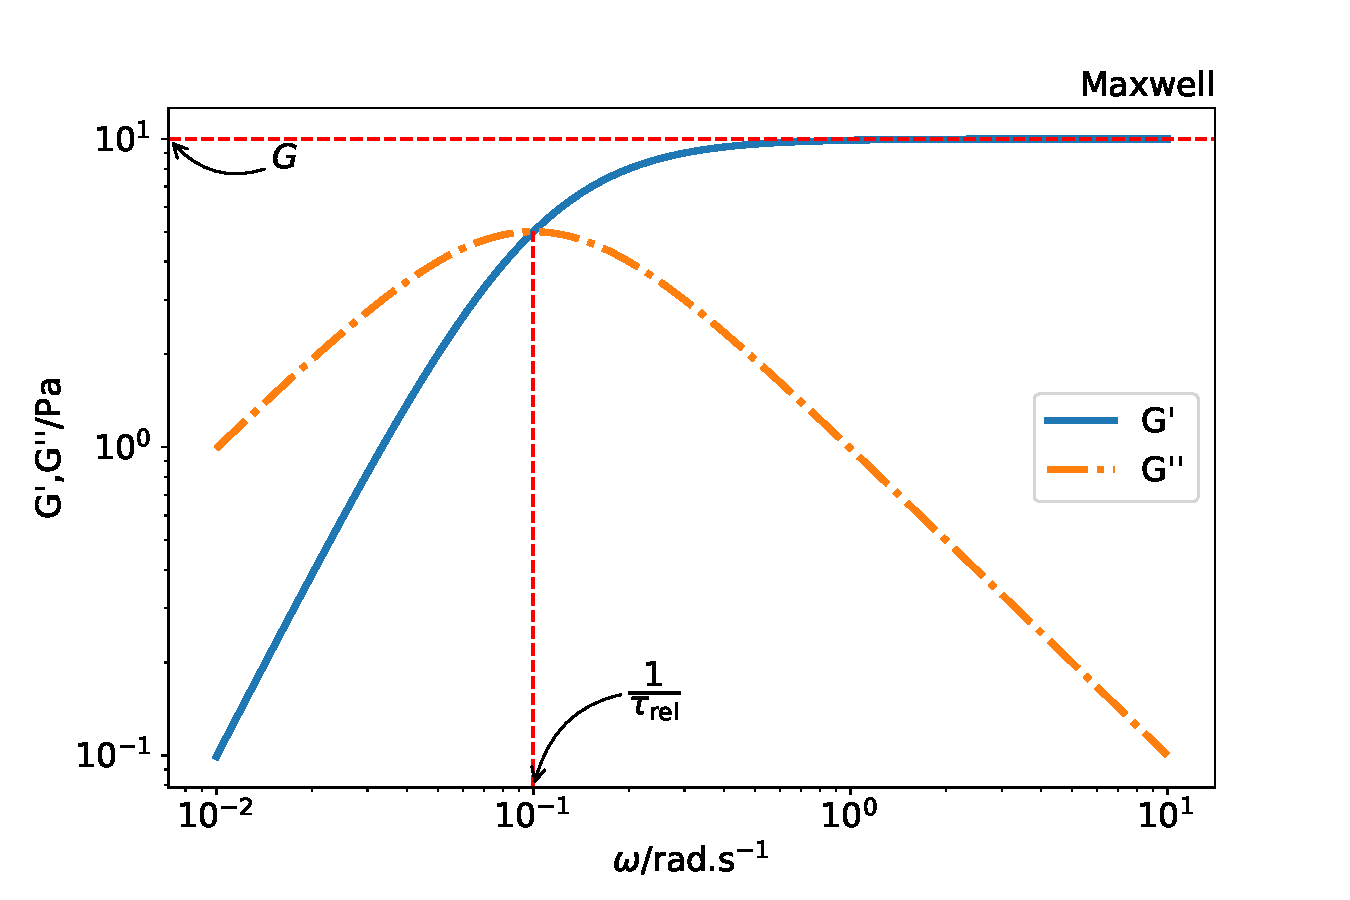
\includegraphics[width=0.7\textwidth]{./imagens/reologia/modelo_maxwell}
				\caption{Espectro mecânico de acordo com o modelo de Maxwell}
				\label{fig:modelo_maxwell}
			\end{figure}
						
			Micelas gigantes, em vários regimes, obedecem muito bem o modelo de Maxwell. É possível interpretar esse comportamento da seguinte maneira. Em baixas frequências de perturbação (longos tempos), as micelas possuem tempo suficiente para deslizar umas pelas outras, então a maior parte da energia fornecida é perdida, logo o módulo viscoso, ou de perda, possui valores altos. Em frequências altas, a rede micelar e os entrelaçamentos conseguem armazenar a energia, não possuindo tempo suficiente para deslizar, então o módulo elástico, ou de armazenamento, é alto. Na região intermediária, ambos os mecanismos estão presentes, parte da energia é perdida e parte é armazenada, sendo que no ponto de cruzamento, exatamente metade da energia é preservada e metade é perdida.
			
			Para a obtenção de valores mais confiáveis para os parâmetros, é necessário realizar um ajuste dessas curvas. Porém, existem duas curvas que são descritas pelos mesmos parâmetros. Ao invés de se fazer dois ajustes e encontrar quatro parâmetros, é ideal realizar um ajuste das duas curvas simultaneamente. Isso pode ser feito minimizando-se um vetor com os resíduos das duas curvas concatenados. Isso pode ser feito utilizando-se, por exemplo, o Excel, com a ferramenta \emph{Solver} para minimizar o resíduo.
			
			\subsection{Modelos mais complexos}
			
			Experimentalmente, existem divergências entre o modelo de Maxwell e os espectros mecânicos dos materiais. Geralmente, essas divergências aparecem devido ao aparecimento de outros  mecanismos de relaxação em frequências mais altas. Para isso, existem alguns modelos que visam corrigir o modelo de Maxwell, afetando principalmente essa região.
			
			Uma possível correção é utilizar dois elementos de Maxwell em série, produzindo um modelo que tem dois tempos de relaxação e dois módulos (Eqs. \ref{eqn:modelo_doismodos_g1}, \ref{eqn:modelo_doismodos_g2}).
			
			\begin{equation}
				G' = \dfrac{ G_1 \omega^2 \tau_{\textrm{rel,1}}^2   }{  1 + \omega^2 \tau_{\textrm{rel,1}}^2      } + \dfrac{ G_2 \omega^2 \tau_{\textrm{rel,2}}^2   }{  1 + \omega^2 \tau_{\textrm{rel,2}}^2      }
			\label{eqn:modelo_doismodos_g1}
			\end{equation}
		
			\begin{equation}
				G'' = \dfrac{  G_1 \omega  \tau_{\textrm{rel,1}}        }{ 1 + \omega^2 \tau_{\textrm{rel,1}}^2 } + \dfrac{  G_2 \omega  \tau_{\textrm{rel,2}}        }{ 1 + \omega^2 \tau_{\textrm{rel,2}}^2 }
			\label{eqn:modelo_doismodos_g2}
			\end{equation}
			
			% todo: a viscosidade do Oldroyd é para isso mesmo?
			
			O modelo de Oldroyd é praticamente idêntico ao modelo de Maxwell, e introduz somente um termo relativo à viscosidade do solvente para altas frequências de G'' (Eq. \ref{eqn:modelo_oldroyd_g2}). G' é inalterado.
			
			\begin{equation}
				G'' =\dfrac{  G \omega  \tau_{\textrm{rel}}        }{ 1 + \omega^2 \tau_{\textrm{rel}}^2 } + \eta_{\infty} \times \omega
				\label{eqn:modelo_oldroyd_g2}
			\end{equation}
			
			O modelo mais diferente do modelo de Maxwell é o modelo de Jeffreys, que possui as seguintes formas:
			
			\begin{equation}
				G' = \dfrac{G \omega^{2} \tau_{\textrm{rel,1}} \left(\tau_{\textrm{rel,1}} - \tau_{\textrm{rel,2}}\right)}{1 + \omega^{2} \tau_{\textrm{rel,1}}^{2}}
				\label{eqn:modelo_jeffreys_g1}
			\end{equation}
			
			\begin{equation}
				G'' = \dfrac{G \omega \tau_{\textrm{rel,1}} \left(\omega^{2} \tau_{\textrm{rel,1}} \tau_{\textrm{rel,2}} + 1\right)}{1 + \omega^{2} \tau_{\textrm{rel,1}}^{2}}
				\label{eqn:modelo_jeffreys_g2}
			\end{equation}
			
			% todo: verificar na literatura essas equações.
			
			A Figura \ref{fig:comparativo_modelos} compara os três modelos mais complexos apresentados com o modelo de Maxwell. 
			
			\begin{figure}[H]
				\begin{subfigure}[t]{.5\textwidth}
					\centering
					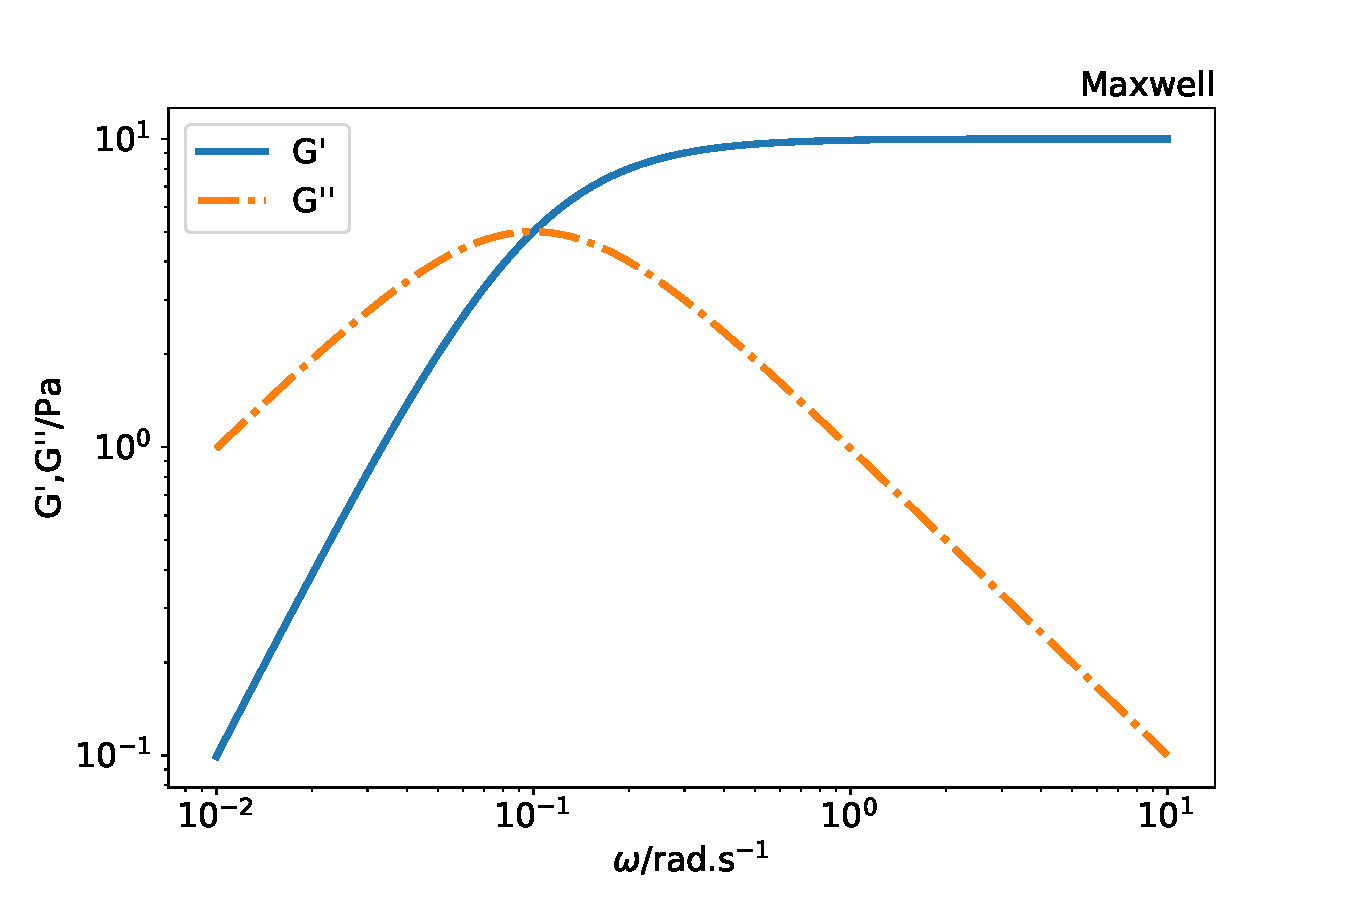
\includegraphics[width=\textwidth]{./imagens/reologia/modelos_comparativo_max}
					\caption{Maxwell. \(G=10, \tau_{\textrm{rel}}=10\)}
					\label{fig:comparativo_modelo_maxwell}
				\end{subfigure}%
				\begin{subfigure}[t]{.5\textwidth}
					\centering
					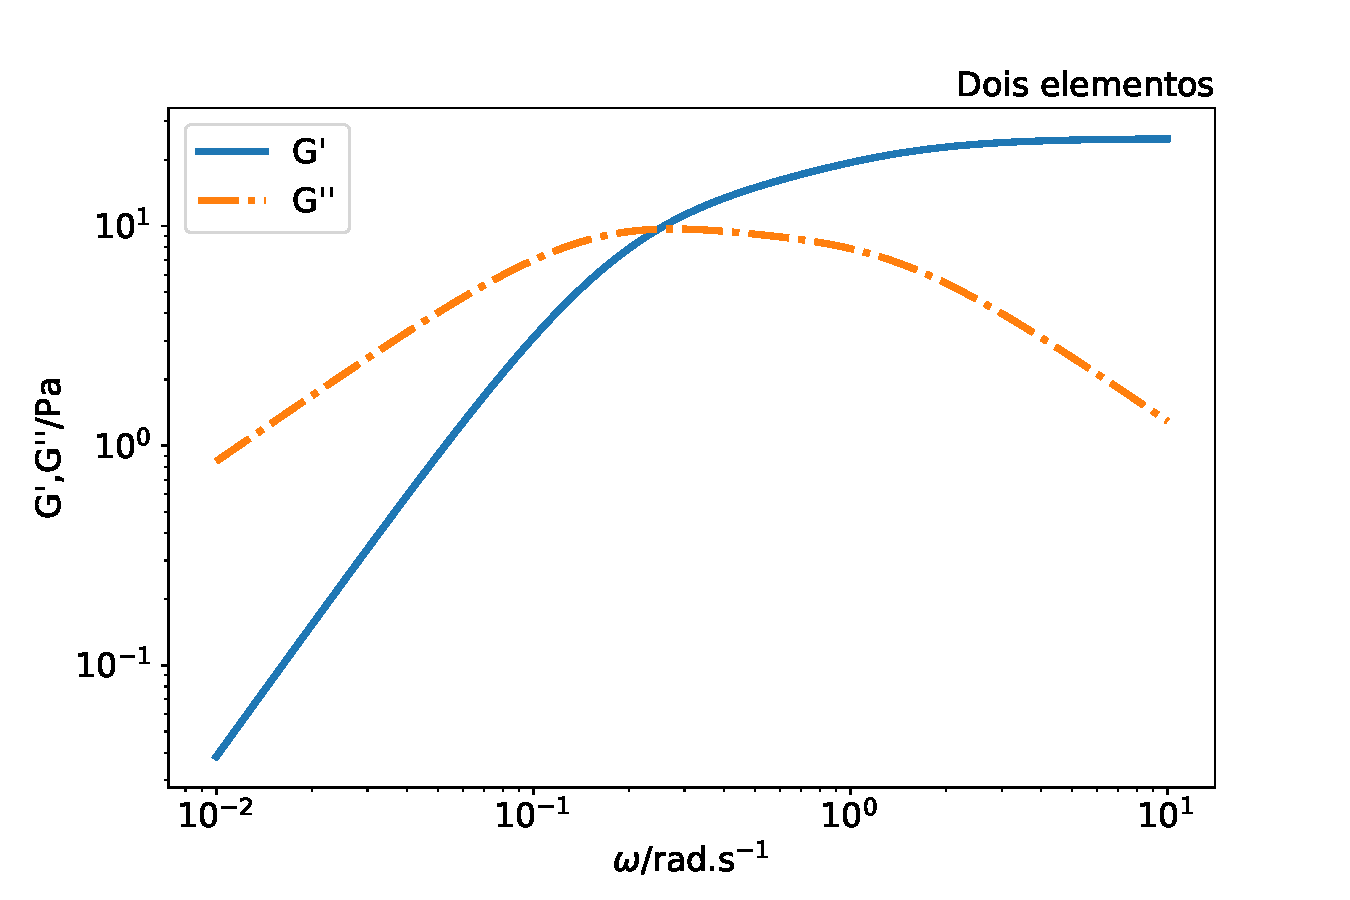
\includegraphics[width=\textwidth]{./imagens/reologia/modelos_comparativo_doismodos}
					\caption{Dois-Modos. \(G_1=10, G=15, \tau_{\textrm{rel,1}}=1,  \tau_{\textrm{rel,2}}=5\)}
					\label{fig:comparativo_modelo_doismodos}
				\end{subfigure}
			
				\begin{subfigure}[t]{.5\textwidth}
					\centering
					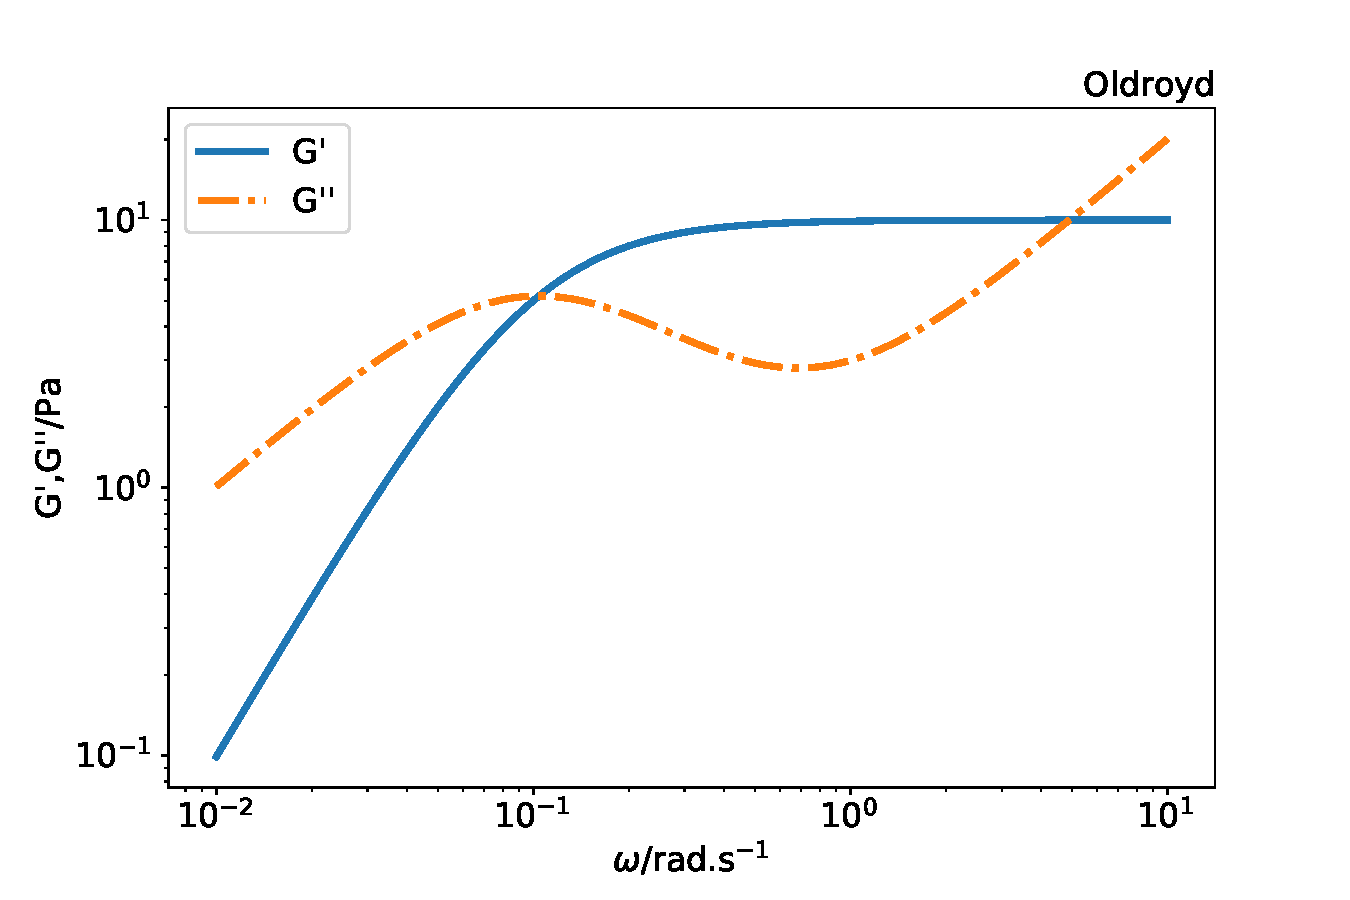
\includegraphics[width=\textwidth]{./imagens/reologia/modelos_comparativo_oldroyd}
					\caption{Oldroyd. \(G=10, \tau_{\textrm{rel}}=10, \eta_{\infty}=2\)}
					\label{fig:comparativo_modelo_oldroyd}
				\end{subfigure}%	
				\begin{subfigure}[t]{.5\textwidth}
					\centering
					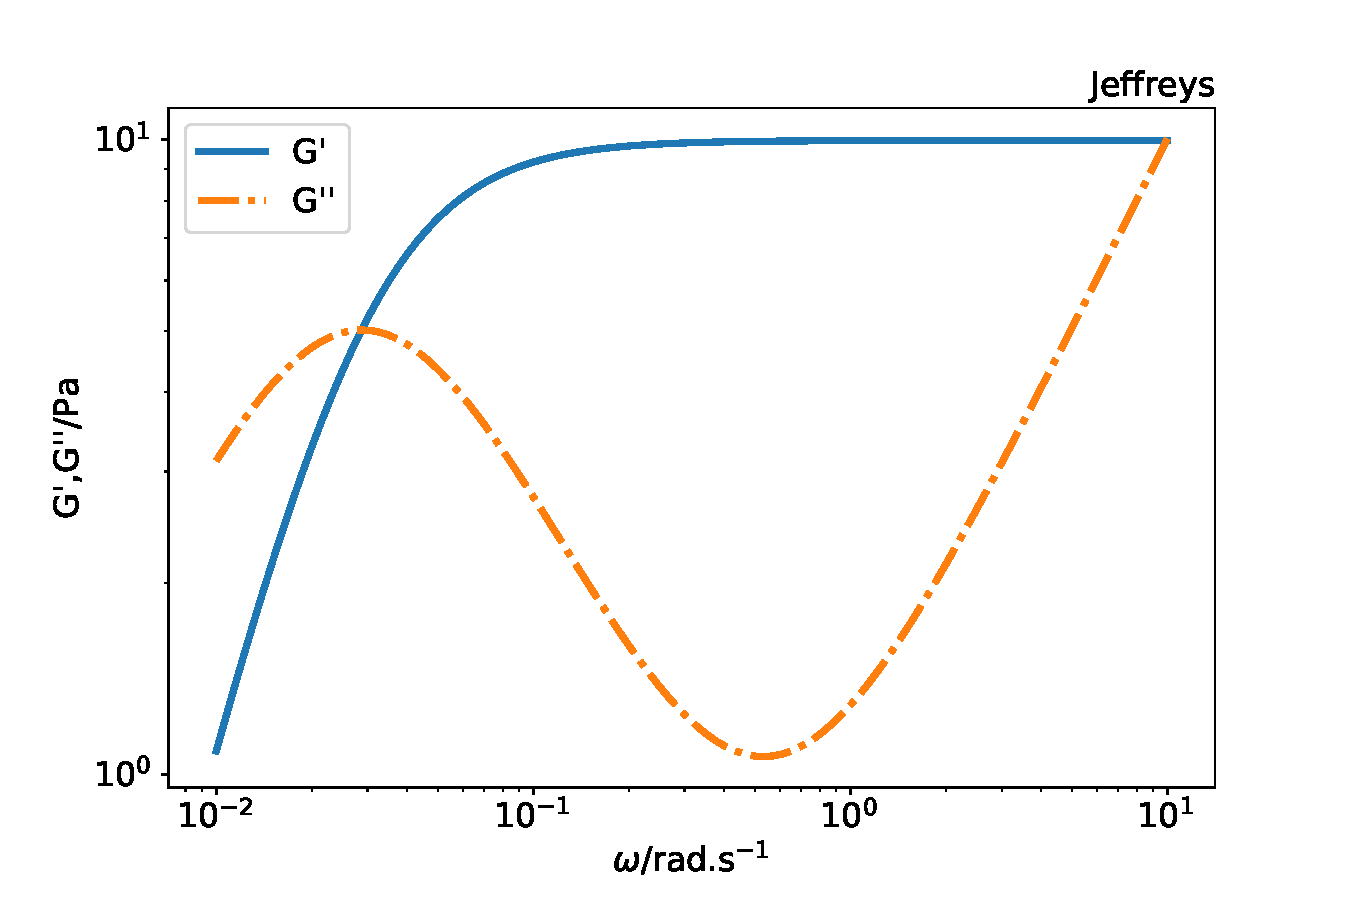
\includegraphics[width=\textwidth]{./imagens/reologia/modelos_comparativo_jeffreys}
					\caption{Jeffreys. \(G=10, \tau_{\textrm{rel,1}}=35, \tau_{\textrm{rel,2}}=0.1 \)}
					\label{fig:comparativo_modelo_jeffreys}
				\end{subfigure}
			
				\caption{Comparação dos modelos de Maxwell, Dois-Modos, Oldroyd e Jeffreys. Nas legendas estão os parâmetros para a criação dos modelos. Os módulos estão na unidade de Pa, os tempos de relaxação, em \(s.rad^{-1}\) e \(\eta_{\infty}\) em Pa.s}
				\label{fig:comparativo_modelos}
			\end{figure}
			
			% todo: pensar se eu devo descrever os detalhes de micelas gigantes aqui, ou na seção de micelas mesmo.
			% todo: colocar o modelo de García-Saraji
	\chapter{Calorimetria de titulação isotérmica}
	
		\section{Fundamentos}
		
		% todo: encontrar um termo melhor para ``caixa adiabática''
		
		A calorimetria de titulação isotérmica (ITC) é uma técnica baseada num processo de titulação, onde cada injeção resulta em uma ou mais reações químicas ou físicas que podem liberar ou absorver calor. O calor total observado é a somatória de todos os processos que ocorreram durante a injeção. No calorímetro há duas celas dentro de uma caixa adiabática, uma de referência, que contém somente água, e outra de amostra, onde ocorre a titulação em si. A cela de referência recebe uma quantidade fixa de calor através de uma resistência, e a cela de amostra recebe uma quantidade variável de calor. Isso significa que a temperatura das celas, no decorrer de uma titulação, aumenta ligeiramente, mas menos que 0,1°C. A figura \ref{fig:ITC_esquema} ilustra a construção de um calorímetro.
		
		\begin{figure}[h]
			\centering
			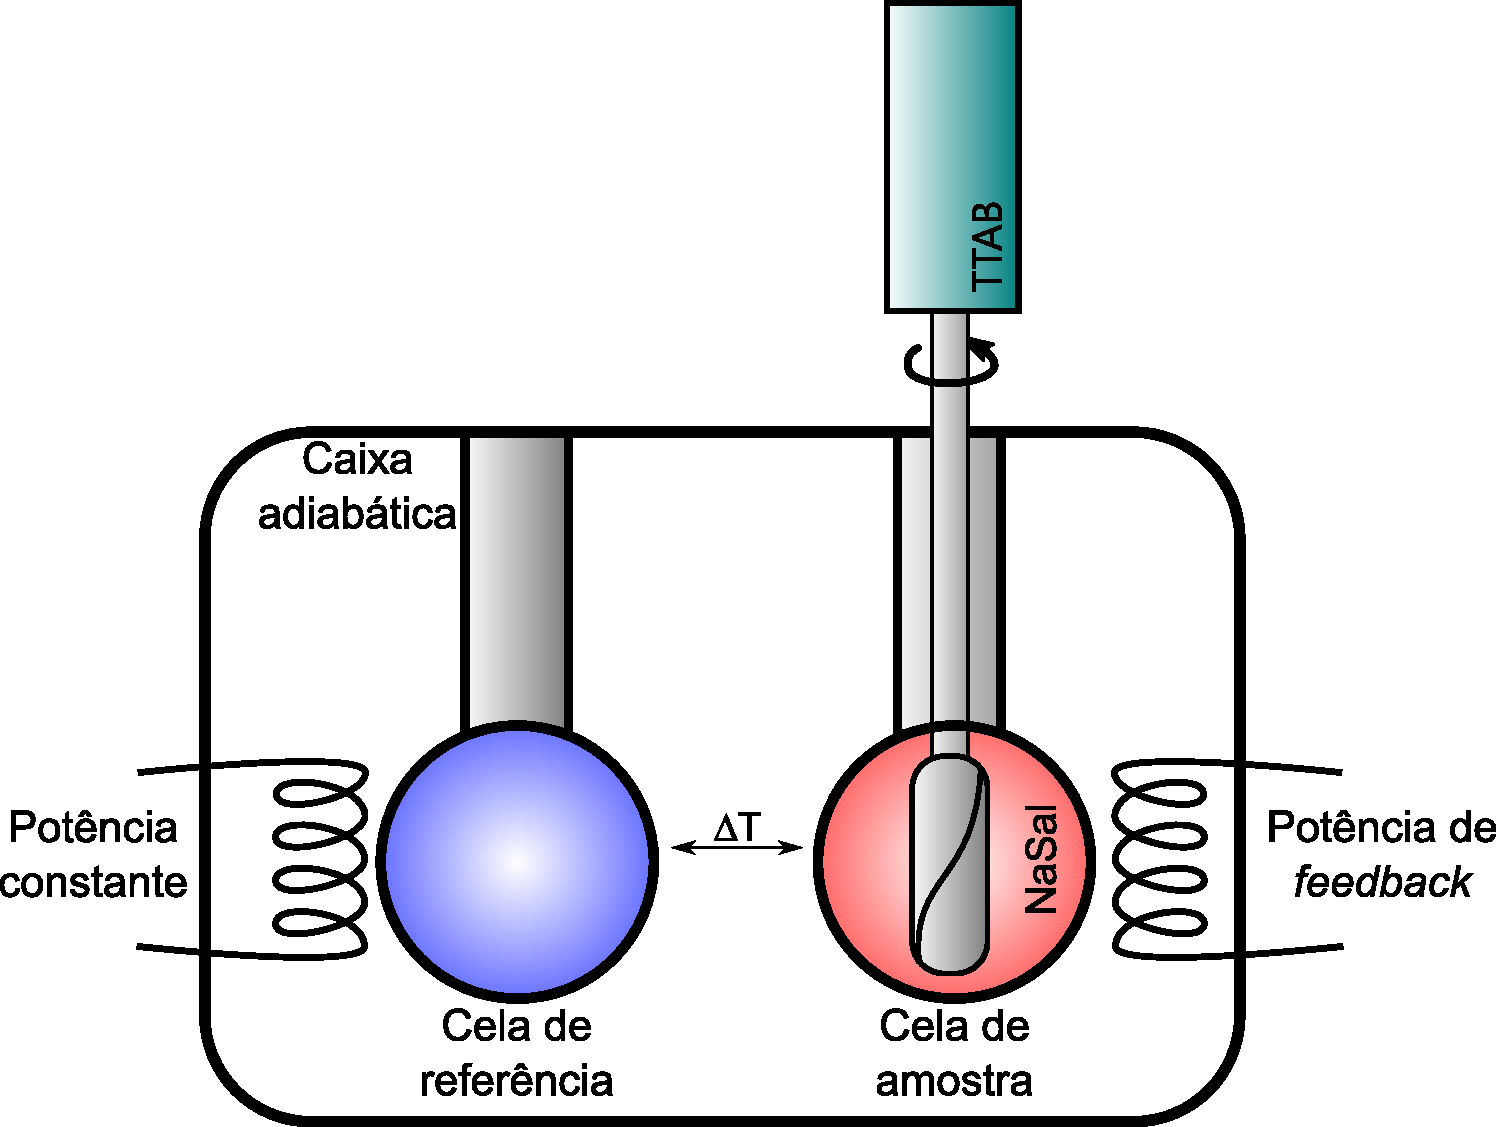
\includegraphics[width=0.5\textwidth]{./imagens/itc/esquema_itc_equipamento}
			\caption{Esquema da construção de um calorímetro de titulação isotérmica}
			\label{fig:ITC_esquema}
		\end{figure}
		
		Durante uma titulação, caso ocorra liberação de calor na cela de amostra, menos energia, em relação ao valor basal, precisa ser fornecida para manter a temperatura igual entre as celas. Caso o sistema absorva energia, mais potência precisa ser fornecida à cela. Esse comportamento se expressa em picos acima ou abaixo da linha de base. A integração de cada pico no tempo fornece valores de energia que, quando divididos pelo número de mols injetados, obtemos valores de $\Delta H^0/kJ.mol^{-1}$ [X, Y]. A figura \ref{fig:ITC_exemplo} mostra um exemplo de um experimento de titulação de \TTAB{} em água.
		
		\begin{figure}[h]
			\begin{subfigure}[t]{0.5\textwidth}
				\centering
				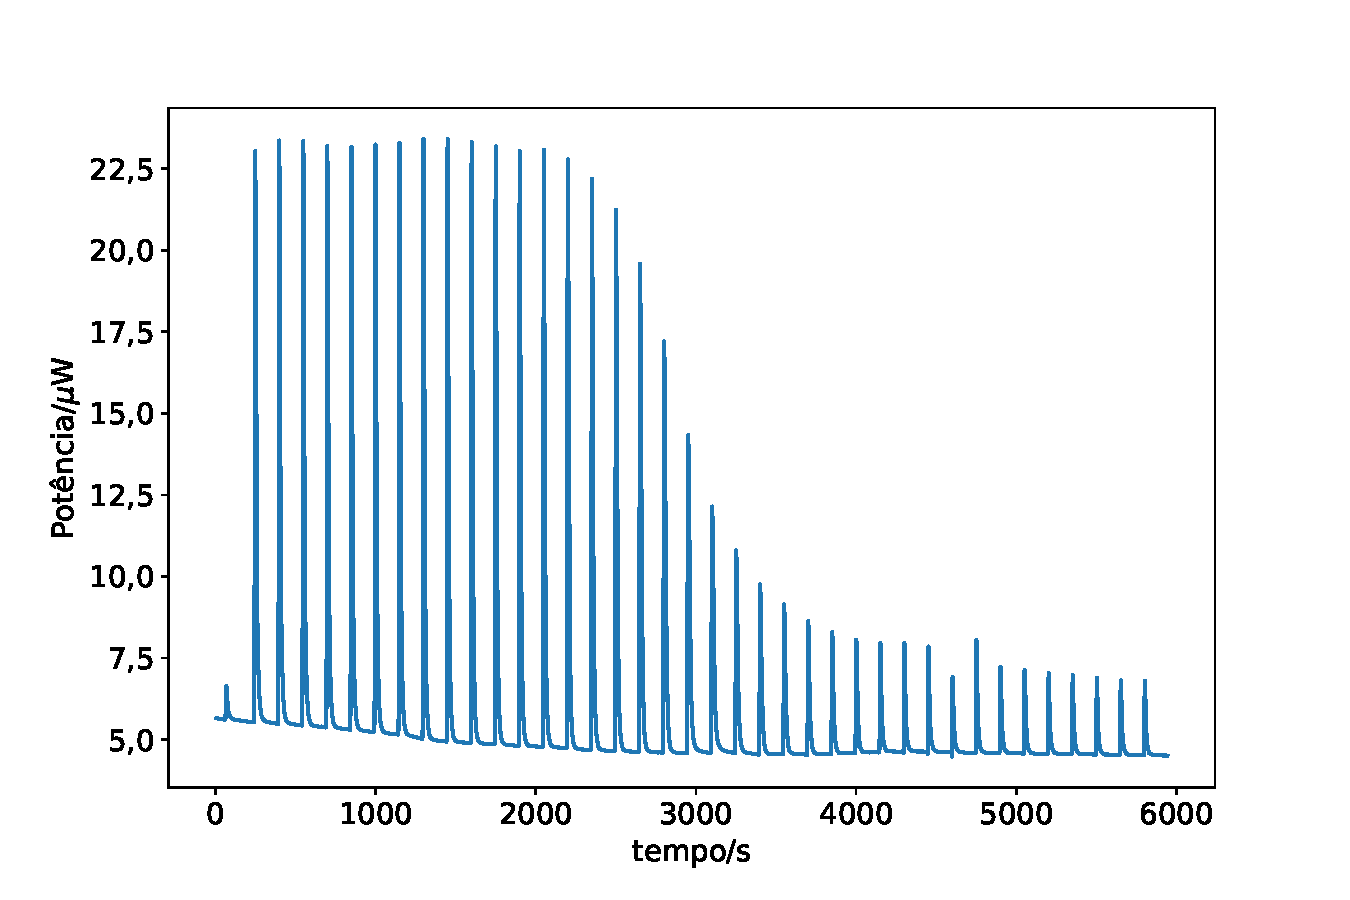
\includegraphics[width=\textwidth]{./imagens/itc/raw_itc_exemplo}
				\caption{Dado bruto}
				\label{fig:ITC_raw_exemplo}
			\end{subfigure}%
			\begin{subfigure}[t]{0.5\textwidth}
				\centering
				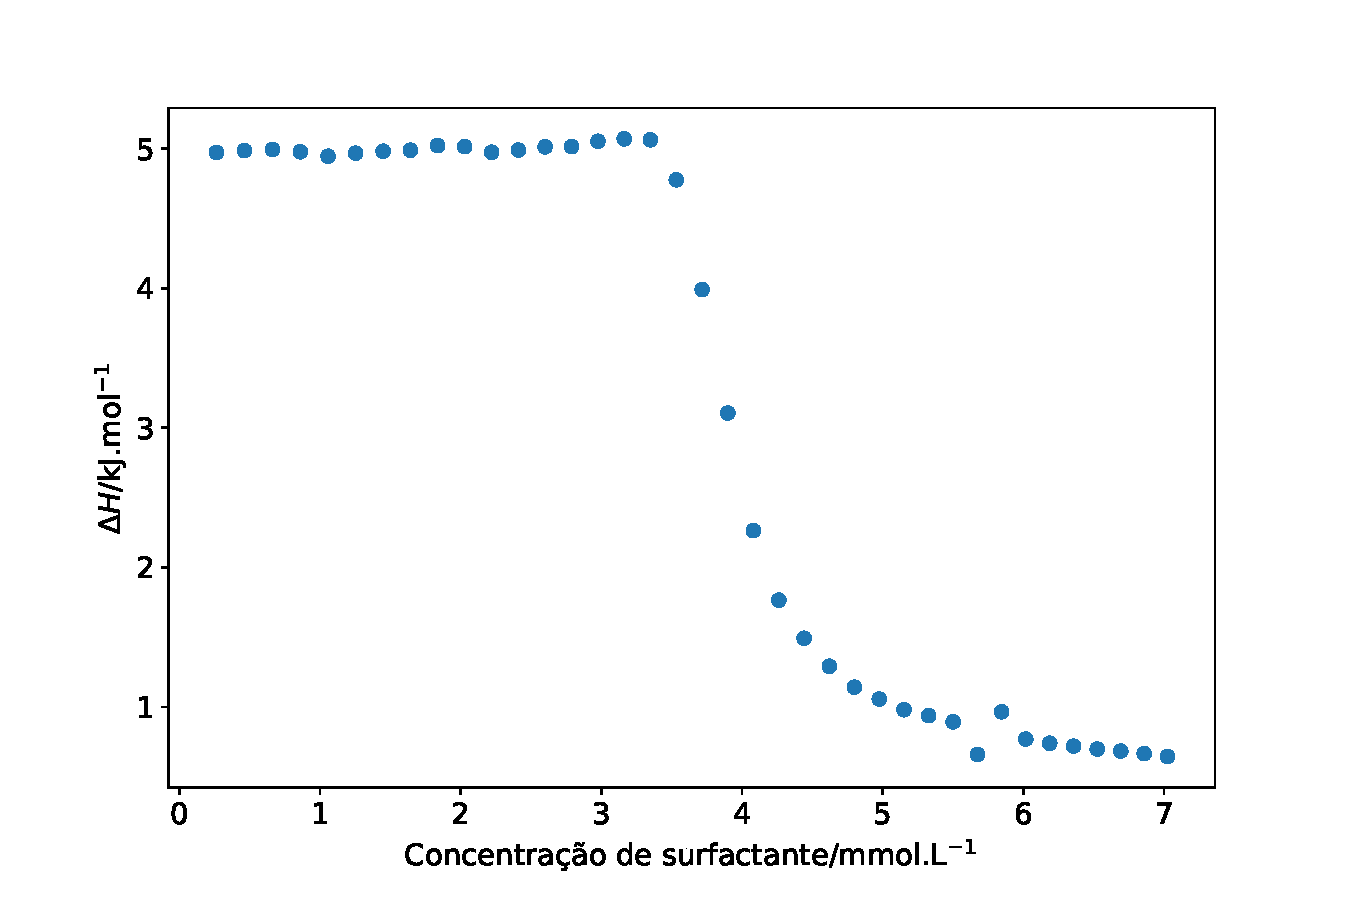
\includegraphics[width=\textwidth]{./imagens/itc/inj_itc_exemplo}
				\caption{Entalpograma}
				\label{fig:ITC_inj_exemplo}
			\end{subfigure}
		
			\caption{Titulação de \TTAB{} 42 \mM{} em água, mostrando o calor absorvido pela célula durante a titulação (\ref{fig:ITC_raw_exemplo}). A primeira injeção é descartada para garantir que as injeções subsequentes possuam um volume correto de injeção. A integração dos picos em relação à linha base, dividindo-se isso pela concentração de surfactante injetado, resulta no entalpograma (\ref{fig:ITC_inj_exemplo})}
			\label{fig:ITC_exemplo}
		\end{figure}
		
		\section{Calorimetria de micelização}
		
		A partir de um conjunto de dados como os da figura \ref{fig:ITC_exemplo}, é possível calcular a \cmc{} e a entalpia de micelização, \DHmic. A \cmc{} é determinada pelo ponto de inflexão, onde a primeira derivada do entalpograma é maior (ou menor). A \DHmic{} é determinada realizando-se dois ajustes lineares das regiões iniciais e finais do entalpograma. A diferença de entalpia dos pontos de intersecção desses ajustes com uma reta horizontal na \cmc{} fornece o \DHmic{} sem correção. Após isso, é necessário corrigir pela concentração de surfactante não micelizado na seringa, que é igual à \cmc{}. A figura \ref{fig:itc_extracao_cmc_dh} mostra esse método.
		
		\begin{figure}[h]
			\centering
			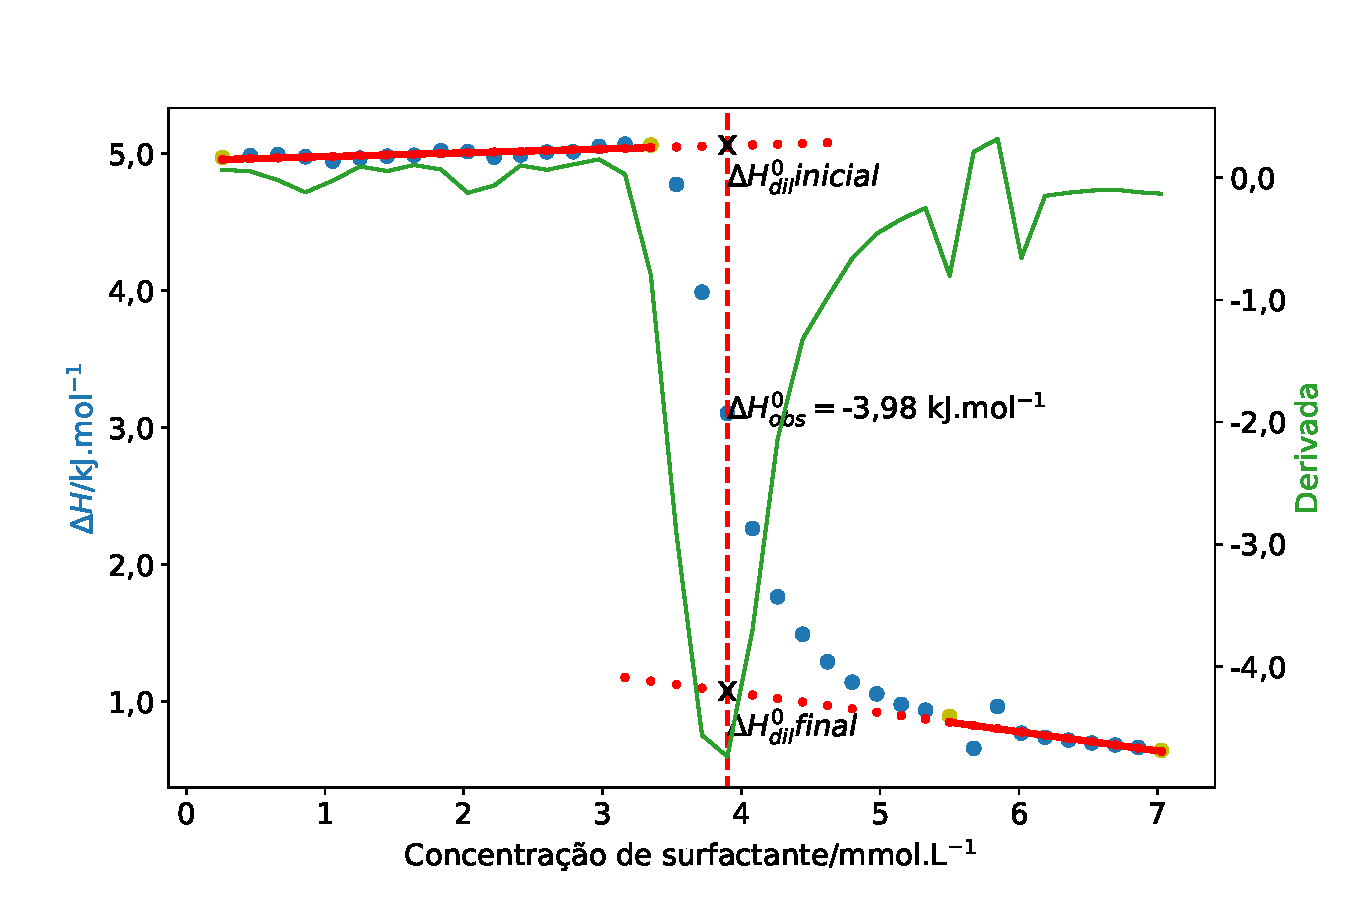
\includegraphics[width=0.7\textwidth]{imagens/itc/extracao_cmc_dh_exemplo}
			\caption{Método para extração da concentração micelar crítica (\cmc) e a entalpia de micelização \DHmic. A curva em verde é a derivada do entalpograma. Os pontos amarelos limitam as regiões onde são feitos ajustes lineares. A }
			\label{fig:itc_extracao_cmc_dh}
		\end{figure}  % todo: checar se as unidades estão corretas

		Para corrigir a entalpia de micelização observada para obter a entalpia de micelização correta, utiliza-se a equação \ref{eqn:itc_obtencao_dhmic}. 
		
		\begin{equation}
			\Delta H^0_{\textrm{mic}} = \Delta H^0_{\textrm{obs}} \times \dfrac{c_{\textrm{seringa}}}{c_{\textrm{seringa}-\textrm{cmc}}}
			\label{eqn:itc_obtencao_dhmic}
		\end{equation}  % todo: ficar de olho aqui porque tem termos que não estão em macros e precisam ser revistos quando algo mudar
		
		\noindent onde \(c_{\textrm{seringa}}\) é a concentração de surfactante na seringa.
		
		Pela \cmc{} é possível obter a energia livre de micelização a partir da equação \ref{eqn:itc_DeltaG_mic}, dependendo do tipo de surfactante e do meio.
		
		\begin{equation}
			\Delta G_{\textrm{mic}}^0
			\begin{cases}
			= RT\ln(\chi_{\textrm{cmc}})      & \textrm{Surfactante não iônico}      \\
			= (2-\alpha)RT\ln(\chi_{\textrm{cmc}}) & \textrm{Surfactante iônico}					\\
			\end{cases}
			\label{eqn:itc_DeltaG_mic}
		\end{equation}
		
		\noindent onde \(\alpha\) é o grau de ionização das micelas e \(\chi_{\textrm{cmc}}\) é a concentração micelar crítica em fração molar. O cálculo para surfactantes iônicos assume que o solvente é água e/ou a força iônica seja baixa.
		
		Com a entalpia e energia livre de micelização, é possível encontrar a entropia de micelização pela equação de Gibbs (Eq. \ref{eqn:itc_gibbs_para_entropia}).
		
		\begin{equation}
			T\Delta S^0_{\textrm{mic}} = \Delta H^0_{\textrm{mic}} - \Delta G^0_{\textrm{mic}}
			\label{eqn:itc_gibbs_para_entropia}
		\end{equation}

		% todo: olhar a dissertação do césar para ver algumas dicas e para colocar alguns termos. Tem bastante coisa boa lá.

	\chapter{SAXS}
		\section{Fundamentos}
				
		%O espalhamento de luz é um fenômeno que ocorre devido à interação da luz com os elétrons de um átomo ou grupo de átomos. O feixe incidente excita os elétrons de modo que eles comecem a oscilar na mesma frequência do feixe incidente. Quando o feixe incidente é removido, os elétrons excitados emitem fótons do mesmo comprimento de onda incidente (chamado de espalhamento elástico), em qualquer direção. As ondas emitidas interagem de maneira construtiva e destrutiva, dependendo de sua posição relativa. A somatória dessas ondas resulta num padrão de espalhamento específico para cada estrutura.
		
		A radiação eletromagnética, quando incide sobre uma amostra fina, o campo elétrico variante da radiação irá interagir com os elétrons dos átomos dentro da região iluminada. Dependendo da frequência (\(\omega\)), pode ocorrer o fenômeno da absorção perto do limite de Lorentz, \(\omega \approx \omega_0\), de interesse em experimentos espectroscópicos, ou pode ocorrer uma polarização dos átomos que varia com a frequência da radiação quando \(\omega \ll \omega_0\) ou \(\omega \gg \omega_0\). Os dipolos emitem radiação pois toda carga elétrica emite um campo elétrico em direções praticamente aleatórias, com amplitude proporcional à aceleração. Isso é chamado de espalhamento. Essas ondas espalhadas interagem construtiva- e destrutivamente, originando em padrões de espalhamento dependendo da localização dos centros espalhadores.
		
		Raios-X possuem comprimentos de onda tão pequenos que se encontram no limite de Thomson, onde \(\omega \gg \omega_0\). No campo da matéria mole, a energia dos fótons é tão alta que todos os elétrons dos átomos, até suas camadas mais internas, oscilam junto com a radiação. Isso não acontece com o espalhamento de luz, onde a oscilação ocorre somente com os elétrons das camadas mais externas, dependendo da polarizabilidade dos átomos, que é proporcional ao índice de refração do material. % todo: pensar se eu coloco aqui a fórmula
		
		As ondas emitidas, quando comparadas com o feixe incidente, são coerentes, isso é, possuem somente uma diferença de fase \(\varphi\) fixa entre a radiação incidente e espalhada, e possuem o mesmo comprimento de onda da radiação incidente, isso é, o espalhamento é completamente elástico. Dessa maneira, os vetores incidentes \(\mathbf{k_i}\) e espalhados \(\mathbf{k_s}\) possuem a mesma amplitude, igual ao número de onda \(k\) (Eq. \ref{eqn:numero_onda}), com o índice de refração próximo à unidade.
		
		\begin{equation}
			k = \dfrac{2 \pi}{\lambda}
			\label{eqn:numero_onda}
		\end{equation}
		
		\noindent onde \(\lambda\) é o comprimento de onda da radiação.
		
		A única diferença entre os feixes espalhados é a fase \(\varphi\) da radiação, devido ao caminho diferente que cada feixe precisa fazer. A diferença de fase de um comprimento de onda é \(2\pi\). Essa fase está relacionada com a interferência dos feixes e, para obtê-la, é necessário subtrair os vetores incidente e espalhado, que passam por um ponto \(P\), cuja posição é dada pelo vetor \(\mathbf{r}\), multiplicados pelo número de onda \(k\) (Eq. \ref{eqn:calculo_fase_saxs}):
		
		\begin{equation}
			\varphi = - \left( \dfrac{2\pi}{\lambda} \right) \mathbf{r} \cdot \left( \mathbf{k_s} - \mathbf{k_i} \right)
			\label{eqn:calculo_fase_saxs}
		\end{equation}
		
		O sinal negativo na equação \ref{eqn:calculo_fase_saxs} é devido à inversão da ordem de subtração dos vetores \(\mathbf{k_i}\) e \(\mathbf{k_s}\). Assim, podemos introduzir o vetor de espalhamento \(\mathbf{q}\), também conhecido como vetor de transferência de momento (Eq. \ref{eqn:vetor_espalhamento}).
		
		\begin{equation}
			\mathbf{q} = \left( \dfrac{2\pi}{\lambda} \right) \mathbf{r} \cdot \left( \mathbf{k_s} - \mathbf{k_i} \right)
			\label{eqn:vetor_espalhamento}
		\end{equation}
		
		Logo, a defasagem pode ser facilmente relacionada com a posição dos centros espalhadores e o vetor de espalhamento:
		
		\begin{equation}
			\varphi = - \mathbf{q} \cdot \mathbf{r}
			\label{eqn:defasagem_qr}
		\end{equation}
		
		Uma consequência do produto escalar da equação \ref{eqn:defasagem_qr} é que somente a componente de \(\mathbf{r}\) na direção de \(\mathbf{q}\) é relevante para a fase \(\varphi\). Isso implica que todos os pontos num plano perpendicular a \(\mathbf{q}\) possuirão a mesma fase. Isso dá origem à ideia de que o espalhamento ocorre como uma reflexão da radiação por um conjunto de planos, comumente utilizado em cristalografia.
		
		A amplitude do vetor de espalhamento é dado pela eq. \ref{eqn:amplitude_vetor_espalhamento}, onde \(\theta\) é o ângulo de espalhamento, entre os vetores \(\mathbf{k_i}\) e \(\mathbf{k_s}\).
		
		\begin{equation}
		q = \dfrac{4\pi}{\lambda} \sin\left(\dfrac{\theta}{2}\right)
		\label{eqn:amplitude_vetor_espalhamento}
		\end{equation}
		
		A figura \ref{fig:esquema_saxs} ilustra os vetores incidente e espalhado, assim como o cálculo do vetor.
		
		\begin{figure}[h]
			\centering
			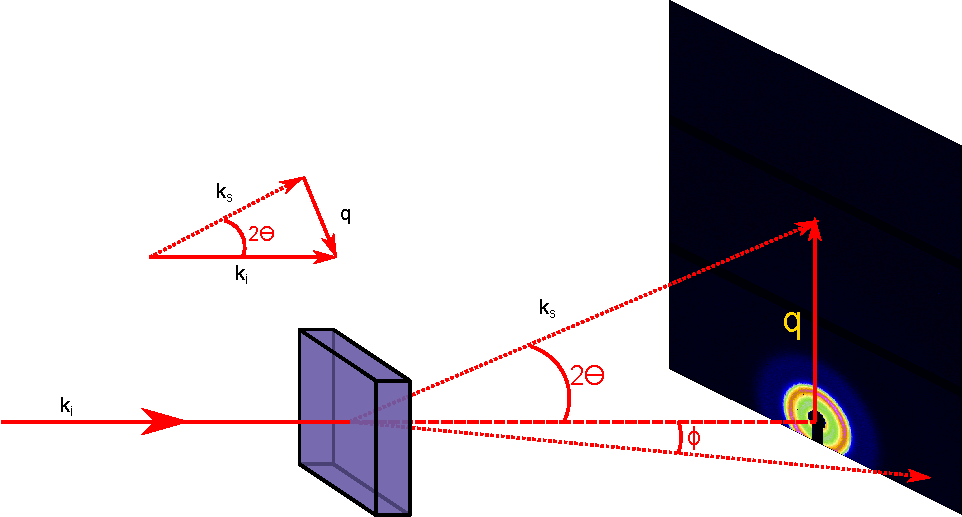
\includegraphics[width=0.7\textwidth]{imagens/saxs/Esquema_SAXS}
			\caption{Diagrama mostrando o feixe incidente de raios-X sendo espalhado por um material, resultando num vetor espalhado. O vetor de espalhamento, \(\mathbf{q}\) é paralelo à subtração vetorial dos vetores \( \mathbf{k_i} \) e \( \mathbf{k_s} \), paralelos à direção dos feixes incidente e espalhado. Os feixes, após interagirem, atingem o detector, e a imagem resultante é composta pela contagem de fótons em cada pixel. O ponto escuro é resultante do bloqueio da radiação não espalhada pelo \emph{beam-stop}.}
			\label{fig:esquema_saxs}
		\end{figure}
		
		Para pequenos valores de \(\sfrac{\theta}{2}\), \(\sin(\sfrac{\theta}{2}) \approx \sfrac{\theta}{2}\), então a magnitude do vetor de espalhamento \(\mathbf{q}\) (que será chamado de \q{} de agora em diante) é proporcional ao ângulo de espalhamento (em radianos). A unidade do vetor de espalhamento é tipicamente \(nm^{-1}\), dependendo claro do comprimento de onda utilizado. Uma grande utilidade de se utilizar o vetor de onda é que o espalhamento se torna independente da fonte de radiação, pois o comprimento de onda já é levado em consideração. Além disso, o inverso de \q{} informa o tamanho dos objetos que geralmente são observados em SAXS. Faixas comuns são de 0,006 a 6 \(nm^{-1}\), o que resulta em estruturas da faixa de 1\(\mu m\) a 1 \(nm\).

		Para se determinar o padrão obtido na figura \ref{fig:esquema_saxs}, é necessário somar todas as ondas espalhadas em cada uma das posições. A função de onda genérica para uma das ondas espalhadas é dada pela Eq. \ref{eqn:funcao_onda_espalhamento}.%, onde \(\mathbf{r}\) é o vetor de posição na partícula.
		
		\begin{equation}
			\psi(\mathbf{q}) = \exp(-i \mathbf{q} \cdot \mathbf{r})
			\label{eqn:funcao_onda_espalhamento}
		\end{equation}
		
		A somatória das funções de onda, Eq. \ref{eqn:SAXS_somatoria_contribs}, resulta na amplitude de espalhamento. O termo \(b_j\) é o comprimento de espalhamento de cada ponto. Para elétrons, seu comprimento de espalhamento é o raio do elétron, \(r_e = 0.2817 \times 10^{-12}\) cm.
		
		\begin{equation}
			A(\mathbf{q}) = \sum_j b_j \exp(-i \mathbf{q} \cdot \mathbf{r})
			\label{eqn:SAXS_somatoria_contribs}
		\end{equation}
		
		Porém, a resolução de raios-X geralmente não permite a observação dos elétrons individuais, então a somatória dos comprimentos de espalhamento de todos os elétrons no átomo, dividido pelo seu volume, resulta na densidade de comprimento de espalhamento \(\rho\) (Eq. \ref{eqn:SLD}). Esse termo também é conhecido como SLD, do inglês \emph{scattering length density}.
		
		\begin{equation}
			\rho(\mathbf{r}) = \sum_j \dfrac{b_j}{v}
			\label{eqn:SLD}
		\end{equation}
		
		Se a densidade for uniforme, podemos encontrar a densidade a partir da fórmula estrutural do material:
		
		\begin{equation}
			\rho = \dfrac{n_e d_M N_a}{M_w} r_e
			\label{eqn:rho_uniforme}
		\end{equation}
		
		\noindent onde \(n_e\) é o número de elétrons do material, \(d_M\) é sua densidade (água é 1000 kg/m\textsuperscript{3}), \(N_a\) é o número de Avogadro, \(M_w\) é a massa molar do material e \(r_e\) é o raio do elétron.
		
		Assim, a eq. \ref{eqn:SAXS_somatoria_contribs} passa de uma somatória para uma integral, eq. \ref{eqn:SAXS_integral_amplitude}.
		
		\begin{equation}
			A(\mathbf{q}) = \int_V \rho(\mathbf{r}) \exp(-i \mathbf{q} \cdot \mathbf{r}) d\mathbf{r}
			\label{eqn:SAXS_integral_amplitude}
		\end{equation}
		
		A intensidade de espalhamento, detectada pelo equipamento, é obtida pela média pelo tempo de todas as posições e conformações possíveis das partículas, ao quadrado (multiplicando-se pelo complexo conjugado). É necessário utilizar constantes para normalizar essa intensidade, como o número \(n\) de partículas espalhadoras e o volume \(V\) das partículas. Além disso, como as partículas estão num meio, como um solvente, é necessário considerar a densidade eletrônica do solvente, e por isso utiliza-se \(\Delta \rho^2\), a diferença entre a densidade do solvente e do meio, também conhecido como contraste. Tudas essas considerações resultam na equação \ref{eqn:SAXS_I_funcao_A}.
		
		\begin{equation}
		I(q) = n\Delta \rho^2 V^2 |A(q)|^2
		\label{eqn:SAXS_I_funcao_A}
		\end{equation}
		
		Sistemas com alto contraste, por exemplo, partículas de ouro em água, espalham bastante raios-X, resultando em sinais de boa qualidade. Porém sistemas de baixo contraste, como a maior parte de sistemas de materia mole, incluindo o sistema \CTAB{} + NaSal, utilizado neste trabalho, não resultam em uma boa resolução sinal/ruído. Tipicamente, o contraste das cabeças é positivo em relação à água, mas o contraste das cadeias é negativo, o que resulta num contraste total baixo. Logo, é interessante calcular o contraste, o que pode ser feito por programas como o SASfit.\footnote{\url{https://github.com/SASfit/SASfit}}. Algumas vezes é possível melhorar o contraste adicionando-se sacarose ou glicerina ao solvente ao meio, porém isso só é válido para experimentos de SAXS, não de espalhamento de luz.
		
		\section{Modelagem e o problema inverso do espalhamento}
		
		O objetivo de análises de SAXS é obter informações estruturais das partículas presentes no meio. Esse é chamado o problema inverso do espalhamento, em contraste com o problema direto, onde estruturas são propostas e o padrão de espalhamento das mesmas é calculado. Para resolver o problema inverso, é necessário primeiramente obter os modelos necessários, um processo matematicamente bastante complexo, e depois ajustá-los às curvas obtidas, variando-se os parâmetros de ajuste pelo método dos mínimos quadrados. A etapa de ajuste também possui seu grau de dificuldade, necessitando frequentemente de técnicas complementares para a escolha de um modelo e para fornecer chutes iniciais para os parâmetros.
		
		\subsection{Partículas esféricas homogêneas em solução}
		
		Quando se considera o espalhamento de um único objeto não centro-simétrico, é necessário considerar a orientação do vetor de espalhamento \q{} para obter o padrão de espalhamento. Além disso, em solução, esses objetos estão possivelmente orientados aleatoriamente, sendo necessário realizar uma integração sobre todas as orientações possíveis. Porém, objetos centro-simétricos, como esferas de raio \(R\), não necessitam disso, e a amplitude de espalhamento pode ser calculada pela eq. \ref{eqn:SAXS_amplitude_esfera}. % Note que foi utilizada a relação de Euler.
		
		\begin{equation}
			A(q) = \dfrac{4\pi\Delta\rho}{q} \int_0^R r\sin(qr) dr
			\label{eqn:SAXS_amplitude_esfera}
		\end{equation}
				
		Realizando uma integração parcial, obtemos:
		
		\begin{equation}
			A(q) = \Delta_\rho \dfrac{4\pi R^3}{3} \left[ \dfrac{3 \left( \sin qR - qR \cos qR \right)}{\left(qR\right)^3} \right]
			\label{eqn:SAXS_amplitude_esfera_integrado}
		\end{equation}
		
		Essa equação, normalizada, é utilizada na descrição do modelo de micelas gigantes (Eq. \ref{eqn:AP_Fsphere}) que está presente no apêndice \ref{sec:modelo_MG_matematica}.
		
		Como a intensidade de luz espalhada é o quadrado da amplitude:
		
		\begin{equation}
			I(q) = (\Delta \rho)^2 V^2 P_0=(\Delta \rho)^2 V^2 \left[ \dfrac{3 \left( \sin qR - qR \cos qR \right)}{\left( qR \right) ^3} \right]
			\label{eqn:SAXS_intensidade_esfera}
		\end{equation}
		
		O termo à direita da equação \ref{eqn:SAXS_intensidade_esfera} é chamado de fator forma normalizado, \(P_0\). Esse fator forma possui vários mínimos em valores de \(qR\) em 4,493, 7,725, etc (figura \ref{fig:espalhamento_esfera}). A partir desses mínimos é possível obter o raio da partícula, apesar de que isso só é válido para partículas monodispersas, totalmente esféricas, homogêneas e em uma solução diluída.
		
		\begin{figure}[h]
			\centering
			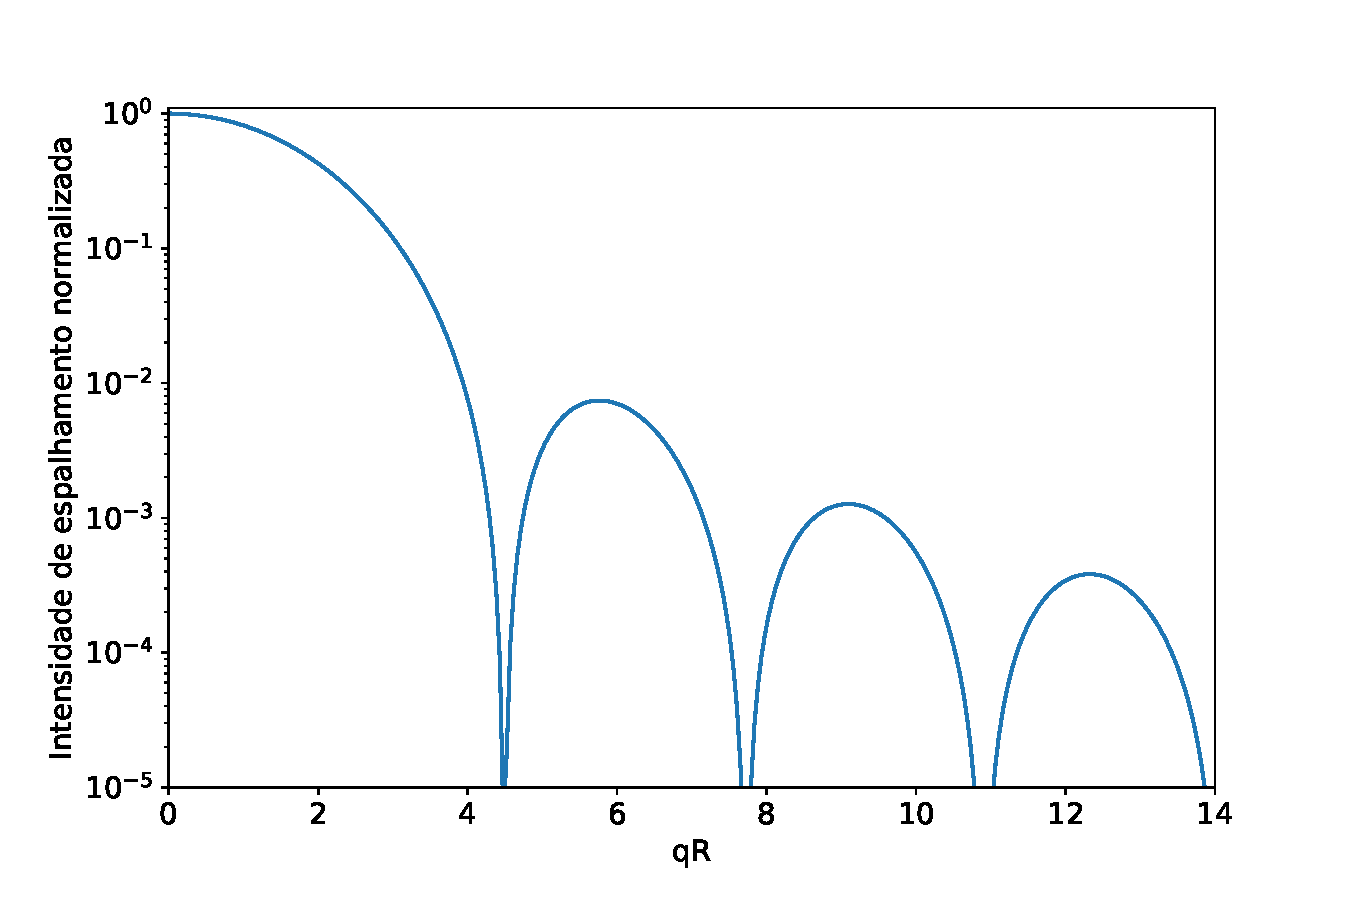
\includegraphics[width=0.7\textwidth]{imagens/saxs/espalhamento_esfera_monodispersa}
			\caption{Espalhamento de uma esfera monodispersa. Os mínimos estão relacionados com o raio da esfera. O código para fazer este gráfico se encontra na listagem \ref{lst:plot_micela_esferica}.}
			\label{fig:espalhamento_esfera}
		\end{figure}
		
		\begin{listing}[H]
			\inputminted{python}{./python/plot_saxs_esfera.py}
			\caption{Código utilizado para a criação da figura \ref{fig:espalhamento_esfera}}
			\label{lst:plot_micela_esferica}
		\end{listing}
		
		Esse é o exemplo mais simples para a derivação da amplitude de espalhamento de um objeto. Quanto maior for a complexidade dos objetos modelados, e mais concentrada for a solução, mais difícil fica a derivação dos modelos, exigindo considerável experiência e conhecimento matemático. O Prof. Jan Skov Pedersen, da Dinamarca, adaptou modelos descritos na literatura para descrever sistemas alongados em solução, como polímeros e micelas gigantes. Uma descrição matemática superficial do modelo desenvolvido se encontra na no apêndice, seção \ref{sec:modelo_MG_matematica}, e uma adaptação desse modelo na linguagem Python se encontra na seção \ref{sec:modelo_MG_python}.
		
		\subsection{Fator estrutura, concentrações altas}
		
		Quando a translação e orientação de uma partícula em solução começa a depender das outras, uma contribuição do espalhamento dessas correlações começa a se tornar visível. Esse fator adicional, chamado de fator estrutura, \(S(q)\), deve ser multiplicado ao \(P(q)\) para se obter o valor da intensidade correta (Eq. \ref{eqn:SAXS_I_P_S}). Em soluções diluídas, a contribuição do fator estrutura se cancela devido à posição e orientação arbitrárias das partículas, então \(S(q) \approx 1\).
		
		\begin{equation}
			I(q) = n\Delta \rho^2 V^2 P(q) S(q)
			\label{eqn:SAXS_I_P_S}
		\end{equation}
		
		% todo: pensar se eu devo colocar uma parte de mínimos quadrados, mostrando exemplo com código, ou Excel também.
		Como as distâncias entre partículas são tipicamente maiores do que as distâncias dentro das partículas, as contribuições do fator estrutura geralmente aparecem com maior intensidade em valores de \q{} baixos.
		
		Existem vários modelos possíveis para o fator \(S(q)\), que dependem de uma função que descreve a probabilidade de se encontrar uma partícula a uma distância \(r\) de outra. Dentro dessa função, existe um potencial que pode descrever, por exemplo, se há atração ou repulsão eletrostática entre as partículas. O modelo das esferas rígidas sem carga, o mais simples, que possui o seguinte potencial (Eq. \ref{eqn:potencial_esfera_rígida}):
		
		\begin{equation}
			u(r) = 
			\begin{cases}
				\infty  & r < (R_a + R_b) \\
				0		& r > (R_a + R_b)
			\end{cases}
			\label{eqn:potencial_esfera_rígida}
		\end{equation}

		\noindent onde \(R_a\) e \(R_b\) são os raios de duas partículas que estão interagindo.
		
		A presença de fatores estrutura adicionam alguns parâmetros fortemente não lineares ao ajuste e aumentam grandemente a complexidade dos mesmos, tornando a determinação do fator forma e estrutura simultaneamente uma tarefa bastante difícil. Além disso, quando há polidispersidade nos sistemas, não se torna possível a completa separação dos termos \(P(q)\) e \(S(q)\) (como é o caso das micelas gigantes do apêndice \ref{sec:modelo_MG_matematica}) e é necessário utilizar um fator estrutura efetivo, \(S_m(q)\).
		
		\subsection{Indexação de picos}
		\label{sec:teoria_SAXS}
		
		Outro exemplo de estruturação é o que ocorre quando existem fases lamelares em solução. Geralmente, os picos oriundos do fator estrutura se superpõem ao fator forma, tornando-se bastante evidentes. Esses picos são consequência da ordenação equidistante das bicamadas, e a posição dos picos está relacionada à distância média das lamelas. Outras mesofases também resultam em fatores estrutura, mas com a posição relativa dos picos em valores diferentes, o que permite a identificação da fase a partir de SAXS. A figura \ref{fig:exemplo_saxs} mostra o padrão de espalhamento de uma amostra lamelar real. Essa figura é resultado da integração azimutal da imagem da figura \ref{fig:esquema_saxs}.
		
		\begin{figure}[h]
			\centering
			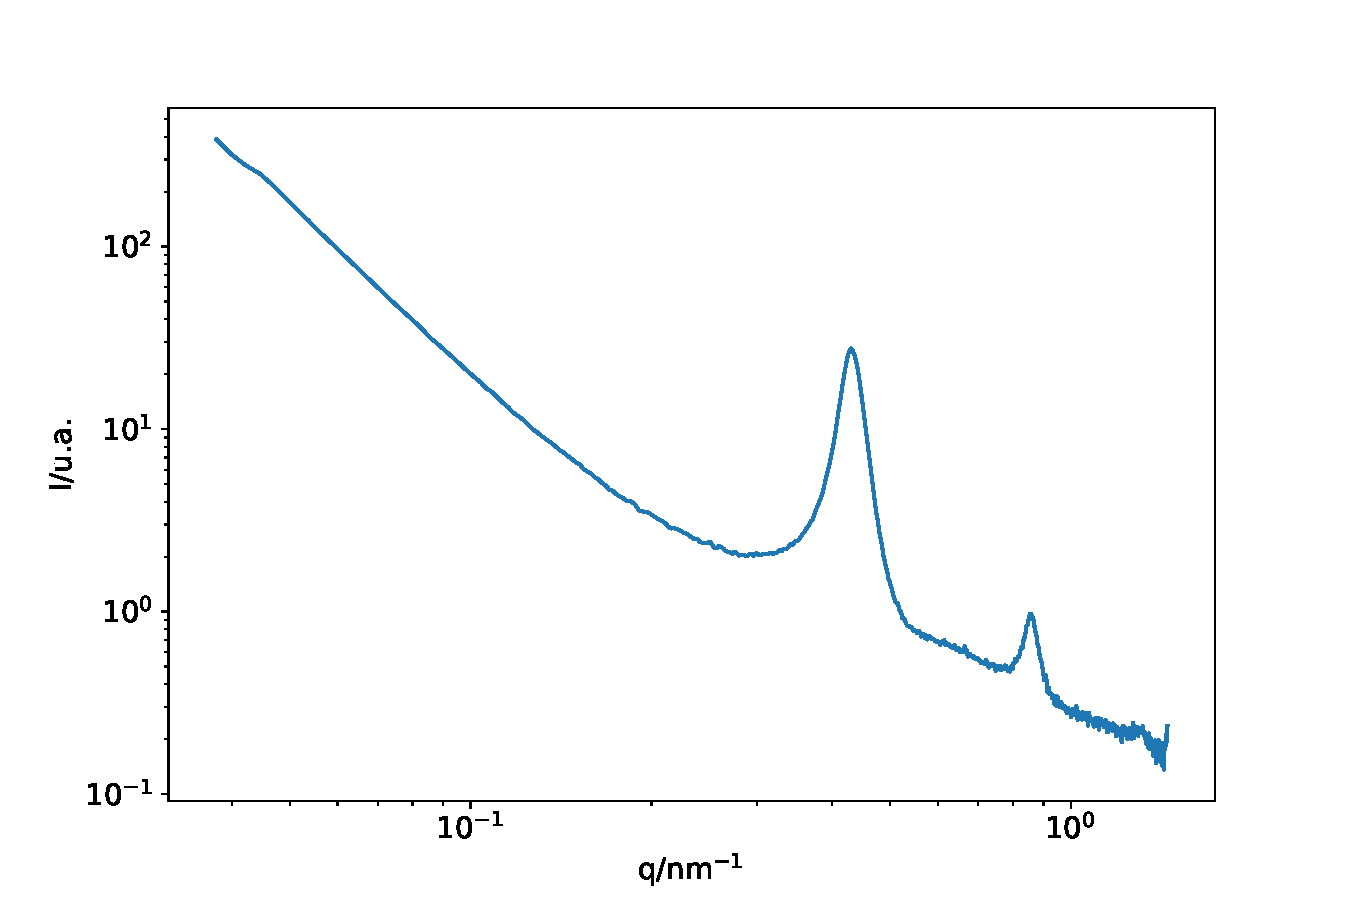
\includegraphics[width=0.7\textwidth]{imagens/saxs/exemplo_SAXS}
			\caption{Curva de espalhamento resultante da integração em \(\phi\) do padrão de espalhamento obtido na fig. \ref{fig:esquema_saxs}. Os picos obtidos nessa figura são resultado da difração de raios-X devido à presença de uma estrutura lamelar em solução.}
			\label{fig:exemplo_saxs}
		\end{figure}
		
		Com o valor de \q{} do primeiro pico, é possível determinar o parâmetro de rede (\emph{lattice parameter}) da mesofase. Para estruturas lamelares, que são de maior relevância para este trabalho, temos que o espaçamento dos picos é de \(1:2:3:4...\). O parâmetro de rede, \(d\), é dado pela Eq. \ref{eqn:SAXS_param_rede_lamela}, e seu significado está ilustrado na figura \ref{fig:saxs_distancia_interlamelar}. É interessante notar a semelhança desse método de identificação com a determinação do raio de esferas pelos mínimos da figura \ref{fig:espalhamento_esfera}. Os picos observados também são chamados de picos de Bragg, mostrando a íntima relação com a área de difração de raios-X, e a modelagem desse tipo de curva de espalhamento utiliza os índices de Miller dos objetos.
	
		\begin{equation}
			q = \dfrac{2\pi}{d}
			\label{eqn:SAXS_param_rede_lamela}
		\end{equation}
		
	
		\begin{figure}[h]
			\centering
			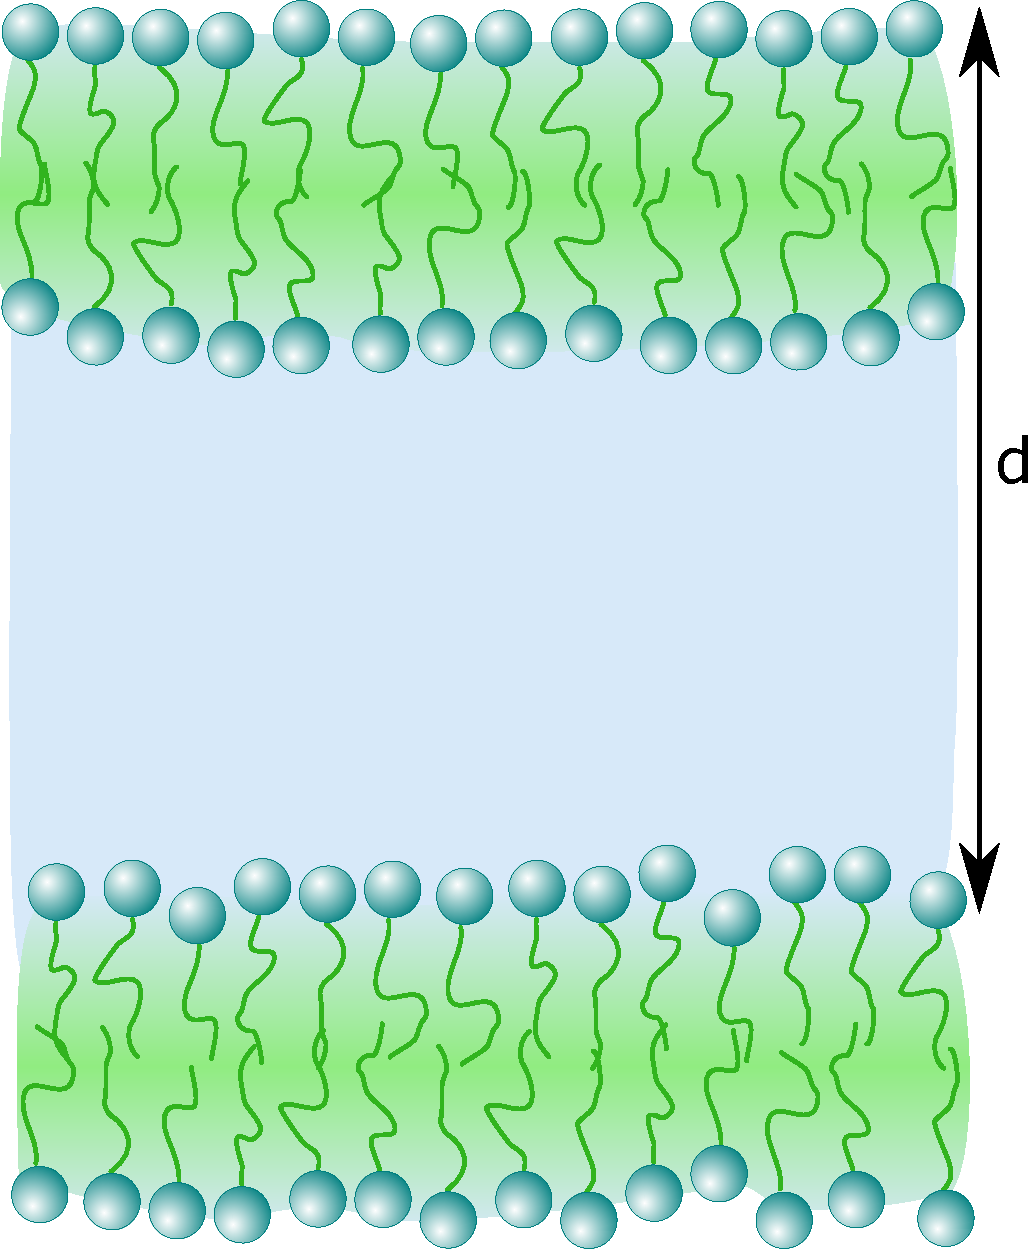
\includegraphics[width=0.35\textwidth]{imagens/saxs/distancia_interlamelar}
			\caption{Distância interlamelar}
			\label{fig:saxs_distancia_interlamelar}
		\end{figure}

		% todo: colocar a referência do artigo do guilherme
		A partir da distância interlamelar, é possível calcular a espessura lamelar (\(d_{\text{HC}}\)) caso a fração volumétrica de surfactante (\(\phi_s\)) e solvente (\(\phi_w\)) também sejam conhecidos. Nesse caso, seria necessário somente relacionar as proporções das regiões com o total, a distância interlamelar. Esse é o princípio do método descrito em X. A fração volumétrica de surfactante pode ser obtida pela Eq. \ref{eqn:SAXS_frac_volum}, cujos parâmetros estão explicados na tabela \ref{tab:ur_fracvol_descr}.
		
		\begin{equation}
			\phi_s = \dfrac{V_{\textit{HC}}\left( \dfrac{w_{s}}{M_{s}} \right)}{\left( V_{\textit{HC}} + V_{P} \right)\dfrac{w_{s}}{M_{s}} + V_{w}\dfrac{w_{w}}{M_{w}}}
			\label{eqn:SAXS_frac_volum}
		\end{equation}
		
	% + V_{\textit{ur}}\dfrac{w_{\textit{ur}}}{M_{\textit{ur}}
	
		\begin{table}[H]
			\IBGEtab{\caption{Descrições das variáveis da equação \ref{eqn:SAXS_frac_volum} \label{tab:ur_fracvol_descr}}}
			{\begin{tabular}{r l}
				\toprule
				           Variável & Descrição                                               \\ \midrule
				              \(s\) & Fração volumétrica de surfactante                       \\
				\(V_{\textit{HC}}\) & Volume molar parcial da cadeia alquílica do surfactante \\
				          \(V_{P}\) & Volume molar parcial da cabeça do surfactante           \\
				          \(w_{s}\) & Fração mássica de surfactante                           \\
				          \(M_{s}\) & Massa molar do surfactante                              \\ \midrule
				          \(V_{w}\) & Volume molar parcial de água                            \\
				          \(w_{w}\) & Fração mássica de água                                  \\
				          \(M_{w}\) & Massa molar da água                                     \\ \bottomrule
			\end{tabular}
			}%
			{}%
		\end{table}

		% todo: colocar como que esses valores podem ser estimados
		
		Sabendo então a fração volumétrica de surfactante, podemos obter a espessura da lamela a partir da distância total pela simples relação da equação \ref{eqn:SAXS_espessura_lamelar}.
		
		\begin{equation} \label{eqn:SAXS_espessura_lamelar}
			d_{\text{HC}} = \phi_s d
		\end{equation}
		
		Em suma, o espalhamento de raios-X em baixos ângulos é uma técnica que permite a obtenção de parâmetros estruturais microscópicos médios do sistema, desde que se conheça qual são as estrutura mais prováveis presentes na amostra. Isso é feito através do ajuste de modelos desenvolvidos pela descrição matemática das estruturas, pelo método dos mínimos quadrados, ou também pela indexação de picos.
		
	\chapter{Fluorescência}
		\section{Diagrama de Jablonski}
		
		O fenômeno de fluorescência é uma subdivisão do fenômeno luminescência, posição que compartilha com a fosforescência. A diferença entre os dois fenômenos está no mecanismo de transição eletrônica, que também altera os tempos de vida dos dois fenômenos. De forma geral, os tempos de vida de fluorescência são da ordem de \(10^{-8} s\), já a fosforescência os tempos de vida variam de milissegundos a segundos. Neste trabalho, somente o fenômeno da fluorescência é de importância.
		
		Uma maneira de se visualizar os fenômenos de luminescência é através do diagrama de Jablonski. Nesse tipo de diagrama, o eixo y representa energia, e as várias linhas representam níveis energéticos. A figura \ref{fig:diagrama_jablonski} mostra um diagrama de Jablonski onde os fenômenos de absorção, fluorescência e fosforescência estão ilustrados. Os níveis \(S\) representam os estados singleto, e seu subíndice representa o nível eletrônico, sendo 0 o fundamental, que é marcado como uma linha mais grossa. Os níveis vibracionais são marcados de 0 a 4 nesse diagrama, com uma linha mais fina. As linhas pontilhadas representam processos não-radiativos e as linhas cheias representam processos radiativos. As cores das linhas são proporcionais aos comprimentos de onda envolvidos, mas não descrevem as cores reais. O nível tripleto é representado como \(T_1\).  % todo: colocar o que é um singleto.
		
		\begin{figure}[h]
			\centering
			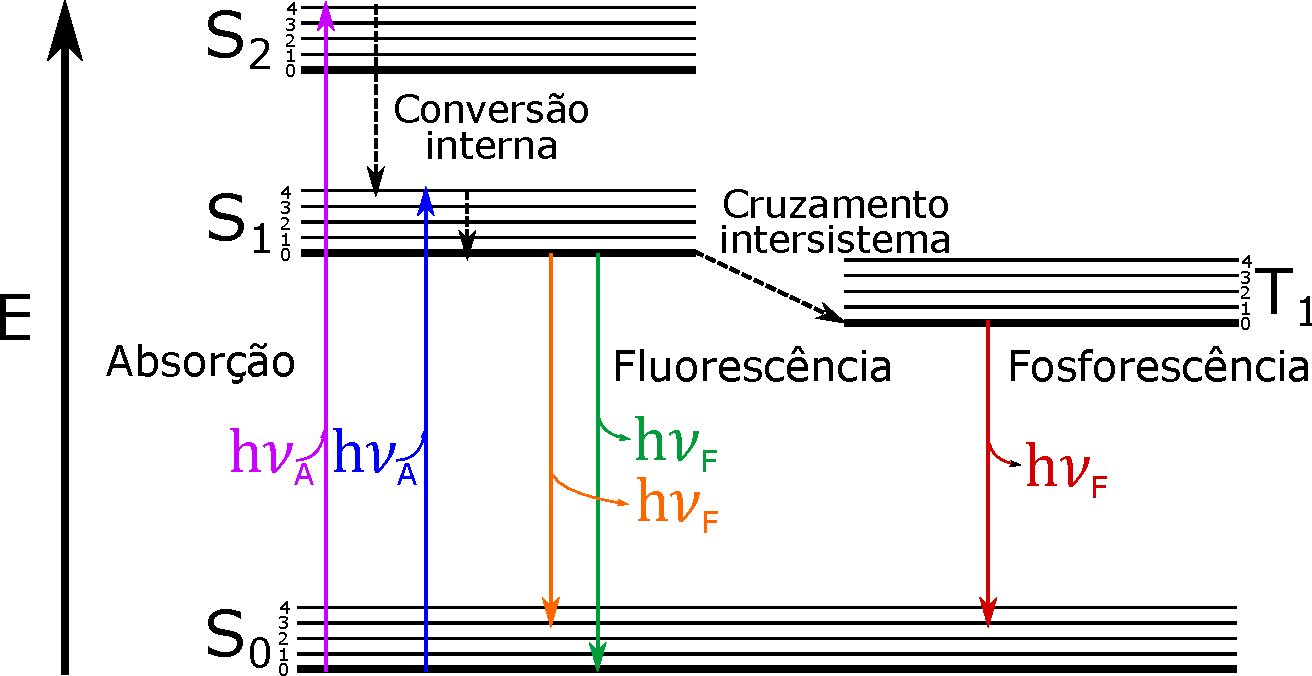
\includegraphics[width=0.7\textwidth]{imagens/fluor/diagrama_jablonski}
			\caption[Diagrama de Jablonski]{Diagrama de Jablonski. As linhas horizontais indicam níveis energéticos, com níveis mais altos para cima. As setas indicam transições radiativas e as setas tracejadas indicam transições não radiativas. As cores das setas são proporcionais à energia de cada transição. Por simplicidade, não estão representados os fenômenos de extinção, transferência de energia e interação com o solvente. Adaptado de X}
			\label{fig:diagrama_jablonski}  % todo: colocar a referência dessa adaptação
		\end{figure}  
		
		\section{Origem do fenômeno de fluorescência}
		
		Quando uma molécula absorve radiação no comprimento de onda adequado, um de seus elétrons passa para um nível eletrônico maior, e geralmente para um nível vibracional maior também. Porém, a temperatura ambiente geralmente não é suficiente para manter esses elétrons em níveis vibracionais altos, então eles relaxam rapidamente (\(10^{-12} s\) ou menos) para o nível vibracional fundamental do nível eletrônico excitado, um processo chamado de conversão interna. Essa conversão pode ocorrer de estados eletrônicos mais elevados também. Como essa escala de tempo é muito menor do que a de fluorescência (\(10^{-8} s\)), os elétrons excitados relaxam completamente sua energia vibracional, atingindo um estado excitado termicamente equilibrado.
		
		Após esse equilíbrio térmico, um elétron pode decair para o nível eletrônico fundamental, tanto para níveis vibracionais elevados ou fundamentais, emitindo um fóton de energia igual à transição. Há uma diferença das energias de absorção e de emissão devido à conversão interna e à tendência de ocorrer transições para níveis vibracionais elevados. Essa diferença de energia resulta num deslocamento no comprimento de onda dos espectros de absorção e emissão, chamado de deslocamento de Stokes.
		
		O fenômeno de conversão interna também implica que o espectro de emissão geralmente é independente do comprimento de onda do fóton incidido, pois o espectro de emissão ocorre sempre do estado vibracional fundamental do estado excitado. Essa regra é conhecida como lei de Kasha.
		
		As transições eletrônicas ocorrem numa faixa de tempo muito rápida, de cerca de \(10^{-15} s\). Esse tempo é muito rápido para que tenha ocorrido mudanças nas posições dos núcleos. Isso é conhecido como o princípio de Frank-Condon. Uma das consequências desse princípio é que a probabilidade de uma transição \(S_1 \to S_0\) é igual à probabilidade de uma transição \(S_0 \to S_1\), o que resulta em espectros de emissão e absorção espelhados. Quando o espelhamento não é observado, é possível que o espectro de absorção possua uma absorção para um segundo estado excitado \(S_2\), onde o elétron relaxa rapidamente. Logo, observa-se o somente as transições espelhadas entre os estados \(S_1\) e \(S_0\).
			
		As transições para os estados excitados ocorrem sem alteração do spin do elétron. Porém, caso o elétron troque de spin, no fenômeno chamado de cruzamento intersistema, o novo estado, um tripleto, não possui uma transição permitida para o estado singleto fundamental. Isso faz com que as escalas de tempo para a transição sejam muito maiores do que a fluorescência, onde a transição é permitida.
		
		\section{Rendimento quântico e tempo de vida}
				
		O rendimento quântico é a eficiência de emissão relativo ao número de fótons absorvidos. Quanto mais próximo de 1 for o rendimento quântico, mais intensa é a fluorescência. O tempo de vida é o tempo em que o fluoróforo permanece em seu estado excitado. Quanto maior for o tempo de vida, mais interações podem ocorrer com moléculas ao redor do fluoróforo, e mais informações podem ser obtidas.
		
		A fluorescência é dependente da polaridade do solvente. Isso ocorre porque, geralmente, o fluoróforo no estado excitado possui um dipolo maior do que no estado fundamental. Isso faz com que as moléculas do solvente ao redor do fluoróforo se rearranjem ao redor dele, diminuindo a energia do sistema, aumentando o deslocamento de Stokes. O rearranjo de uma molécula de solvente ocorre na ordem de 40 ps ou menos, e o rearranjo total ocorre em cerca de \(10^{-10} s\). Dependendo da polaridade do solvente, os efeitos do rearranjo podem ser maiores ou menores, resultando em deslocamentos de Stokes diferentes e espectros de emissão de fluorescência deslocados.
		
		Na área de fluorescência existem dois métodos experimentais, a fluorescência estacionária e a fluorescência resolvida no tempo. Na fluorescência estacionária, a amostra é iluminada e observada constantemente. Como os fenômenos de fluorescência são muito rápidos, efetivamente observa-se uma média dos fenômenos que ocorreram durante a observação. Utilizando equipamentos bastante sofisticados, é possível emitir pulsos de radiação curtos e observar o decaimento da fluorescência com o tempo, em escalas de ns. Isso é conhecido como fluorescência resolvida no tempo. Neste trabalho, foi utilizado somente fluorescência estacionária e, de certo modo, uma combinação das duas técnicas, onde observou-se a variação de fluorescência em escalas de ms a minutos.
		
		% todo: colocar as equações para rendimento quÂntico e tempo de vida?
		
		\section{Extinção}
		
		Há fenômenos que conseguem impedir uma molécula de fluorescer, diminuindo a intensidade de fluorescência medido. Esses fenômenos são chamados de extinção (\emph{quenching}). Há pelo menos três mecanismos possíveis para a extinção:
		
		\begin{enumerate}[noitemsep]
			\item Troca eletrônica
			\item Cruzamento intersistemas, ou o efeito do átomo pesado
			\item Transferência eletrônica fotoinduzida.
		\end{enumerate}
		
		Para a extinção ocorrer, é necessário que haja contato entre a molécula do fluoróforo e do \emph{quencher}. No caso de troca eletrônica, há uma molécula que é pobre eletronicamente, chamada de aceptor e o fluoróforo, o doador. Entrando em contato, o doador transfere seu elétron excitado para o aceptor e recebe de volta um elétron no estado fundamental, concertadamente ou não. Isso equilibra as cargas no sistema, e faz com que o aceptor esteja no estado excitado. O aceptor em seguida pode tanto perder a energia por processos radiativos quanto não-radiativos. % todo: pode mesmo por porcesso radiativo?
		% todo: colocar exemplos aqui
		
		O cruzamento intersistemas, mecanismo que também dá origem à fosforescência, pode ser induzido por átomos pesados, como halogênios, devido ao acoplamento spin-órbita. Em solução aquosa, um elétron no estado \(T_1\) relaxa por processos não radiativos pois o tempo de vida desse tipo de transição é muito alto. O oxigênio é um \emph{quencher} bastante comum e consegue extinguir a maior parte dos fluoróforos, sendo que em alguns casos é necessário removê-lo do meio para permitir a observação de fluorescência. O mecanismo de atuação do oxigênio ainda é debatido, porém o mais provável é que o oxigênio, paramagnético, causa um cruzamento intersistema, e o sistema depois perde energia não radiativamente. Outros estudos mostram que podem existir vários mecanismos em conjunto atuando, como, além do cruzamento, transferência de carga e troca eletrônica. % todo: colocar aqui um artigo que fala do brometo em micelas de CTAB
		
		A transferência eletrônica é resultante da formação de um completo entre um doador e um aceptor eletrônico (o fluoróforo pode ser ambos), formando um complexo do tipo \(D_p^+A_p^-\), que pode voltar ao estado fundamental sem emissão, porém em alguns casos é observada a emissão desse complexo. Após a relaxação, o elétron é retornado ao doador. 
		
		Outro parâmetro que pode influenciar a fluorescência é a viscosidade do meio onde o fluoróforo se encontra. Isso depende da estrutura e do mecanismo de emissão específico de cada fluoróforo. A molécula CCVJ possui um aumento de seu rendimento quântico com o aumento da viscosidade do solvente, em soluções de etileno glicol em glicol. Isso ocorre porque a maior viscosidade atrasa a rotação interna de certos grupos em sua estrutura e dificulta um mecanismo de transferência de carga que extingue a fluorescência, aumentando então o rendimento quântico.
		
		% 	Outra consequência do princípio de Frank-Condon é que o fenômeno de absorção, muito rápido, só fornece informações sobre o estado fundamental médio das moléculas e das moléculas de solvente nas imediações. Porém, como a fluorescência é mais demorada, é possível que ocorram interações com outras moléculas em solução, fornecendo informações sobre o ambiente químico do fluoróforo.
		
		% todo: colocar como se calcula singleto e tripleto.
		
	\chapter{Forças intermoleculares e interagregados}
	
	Na natureza existem quatro forças distintas, porém, para o campo dos coloides, a força eletromagnética é de maior importância. As forças comumente estudadas na química, como as interações dipolares, e dispersivas, possuem uma origem fundamentalmente eletrostática. De forma geral, potenciais de interação de pares \(w\) podem ser escritos de acordo com a equação \ref{eqn:energia_livre_generica}. A força \(F\) é obtida pela derivada dessa equação em função da posição (eqn. \ref{eqn:forca_generica}).
	
	\begin{equation}
		w(r) = -\dfrac{C}{r^n}
		\label{eqn:energia_livre_generica}
	\end{equation}
	
	\begin{equation}
		F(r) = -\dfrac{\mathrm{d}w(r)}{\mathrm{d}r} = -n \dfrac{C}{n+1}
		\label{eqn:forca_generica}
	\end{equation}
	
	\noindent onde \(C\) é uma constante de interação, \(r\) é a distância e \(n\) é um fator de distância.
	
	As interações intermoleculares possuem valores de \(n\) entre 4 e 5. Isso permite que não seja necessário considerar o sistema como um todo para calcular as interações intermoleculares, pois as energia de interação decaem rapidamente, sendo efetivas somente em curtas distâncias. Mie propôs uma forma para o potencial de interação adicionando um componente repulsivo, a equação \ref{eqn:forca_mie}.
	
	\begin{equation}
		w(r) = -\dfrac{A}{r^n} + \dfrac{B}{r^m}
		\label{eqn:forca_mie}
	\end{equation}
	
	\noindent onde \(A\) e \(B\) são as constantes de interação atrativa e repulsiva, respectivamente, e \(n\) e \(m\) são os fatores de distância. O potencial de Lennard Jones ocorre quando \(n = 6\), correspondente às atrações de van der Waals, \(m = 12\). Os valores comuns de \(A\) e \(B\) são \(10^{-77}\) J e \(10^{-134}\) J. % todo: isto é no vácuo?
	
	Quando as interações intermoleculares ocorrem através de um meio, como um solvente, é necessário incluir o efeito das moléculas do solvente nos potenciais de interação. Atrações que seriam previamente atrativas podem se tornar repulsivas num solvente, caso a energia necessária para remover as moléculas de solvente excede a energia de aproximação molecular. Além disso, a presença de moléculas de solvente podem alterar propriedades das moléculas de soluto, como seus momentos de dipolo.
	
	Os valores de energia somente serão úteis se comparados com outros fatores, por exemplo, a energia térmica, que age de modo a equilibrar o sistema e afastar as moléculas. A 1 atm, o valor da energia térmica do solvente é de \(\approx \sfrac{3}{2} kT\), onde \(k\) é a constante de Boltzmann e \(T\) é a temperatura, então interações com energias menores que \(\sfrac{3}{2}kT\) não conseguem so sobrepor ao movimento térmico das moléculas. % todo: ler essa parte e ver se é kT ou 3/2 kT.
	
	As interações intermoleculares possuem três origens distintas:
	
	\begin{enumerate}[noitemsep]
		\item Origem puramente eletrostáticas, como no caso de interações entre íons, dipolos (e quadropolos, etc) permanentes, e interações de polarização.
		\item Origem puramente entrópica, que surgem do comportamento coletivo das moléculas, como as forças osmóticas.
		\item Origem mecânico quântica, como as ligações covalentes, forças de dispersão de van der Waals, ácido-base, forças estérica repulsivas devido ao princípio de exclusão de Pauli.
	\end{enumerate}
	
	\section{Interações Coulombicas}
	
	As interação Coulombica depende do campo elétrico entre uma partícula carregada e a carga de outra partícula próxima. O campo elétrico é dado pela equação \ref{eqn:campo_eletrico}.
	
	\begin{equation}
		E = \dfrac{Q_1}{4\pi\varepsilon_0\varepsilon r^2}
		\label{eqn:campo_eletrico}
	\end{equation}

	\noindent onde \(Q_1\) é a carga da partícula, \(\varepsilon_0\) é a constante dielétrica do vácuo e \(\varepsilon\) é a constante dielétrica relativa do meio em questão. Como pode ser visto, a presença de um meio diminui a força da interação eletrostática por \(\varepsilon\), então em solventes com constantes dielétricas altas, a força eletrostática é bastante enfraquecida. É necessário enfatizar que os termos \(\varepsilon\) e \(\varepsilon_0\) são dependentes da frequência \(\nu\) do campo elétrico aplicado (por exemplo, o campo elétrico oscilatório da luz). Em frequência zero, em condições estáticas, esses termos recebem o nome de constante dielétrica, mas fora dessas condições recebem o nome de permissividade elétrica.
	
	O potencial de interação entre cargas é obtido pelo processo oposto da equação \ref{eqn:forca_generica}, ou seja, pela integração da força eletrostática, dada por \(F = Q_2 E\) (eqn. \ref{eqn:potencial_eletrostático}), utilizando o estado de referência das cargas como sendo no infinito.
	
	\begin{equation}
		w(r) = \int_\infty^r -F(r)dr = \dfrac{z_1z_2e^2}{4\pi\varepsilon_0\varepsilon r}
		\label{eqn:potencial_eletrostático}
	\end{equation}
	
	Interessantemente, a força gravitacional e a interação Coulombica são comparáveis pois possuem um potencial da forma \(1/r\), portanto são de longo alcance, e também são aditivas, isso é, a interação entre dois corpos não é dependente da presença de outras moléculas ao redor. Esse conceito é importante, pois as interações de van der Waals, de grande relevância para coloides, não são aditivas. % todo: ver se é v.d.W. ou se é dispersiva só.
	
	\section{Interações dipolares}
	
	A maioria das moléculas não possui uma carga, mas sim um momento de dipolo, resultante da posição de cargas totais ou parciais em diferentes pontos da molécula. O momento de dipolo é definido como:
	
	\begin{equation}
		u = ql
		\label{eqn:momento_dipolo}
	\end{equation}
	
	\noindent onde \(u\) é o momento de dipolo e \(l\) é a separação entre as cargas \(+q\) e \(-q\). Essas cargas não precisam estar alinhadas, sendo necessário então corrigir esse não alinhamento pela soma vetorial dos momentos de dipolo individuais.
	
	A energia de interação entre duas moléculas dipolares (sendo uma delas fixa) é dada pela equação \ref{eqn:energia_dipolo_dipolo}.
	
	\begin{equation}
		w \left( r , \theta _ { 1 } , \theta _ { 2 } , \phi \right) = - \frac { u _ { 1 } u _ { 2 } } { 4 \pi \varepsilon \varepsilon _ { 0 } r ^ { 3 } } \left[ 2 \cos \theta _ { 1 } \cos \theta _ { 2 } - \sin \theta _ { 1 } \sin \theta _ { 2 } \cos \phi \right]
		\label{eqn:energia_dipolo_dipolo}
	\end{equation}
	
	\noindent onde \(\theta_{ 1 }\) e \(\theta_{ 2 }\) são os ângulos das duas moléculas dipolares em relação à reta que as liga, \(\phi\) é o ângulo de rotação perpendicular a \(\theta_{ 2 }\) de uma das moléculas. É interessante ver que essa interação também é dependente da constante dielétrica, além de ser dependente de \(r^{-3}\).  % todo: pensar se eu devo deixar essa equação ou só colocar a de Keesom
	
	Se os dois dipolos puderem rodar livremente, a energia média dessa interação, conhecida como energia de Keesom é dada por:
	
	\begin{equation}
		w(r) = - \dfrac{u _ { 1 } ^ { 2 } u _ { 2 } ^ { 2 } }{ 3 \left( 4 \pi \varepsilon \varepsilon _ { 0 } \right) ^ { 2 } k T r ^ { 6 } }
		\label{eqn:energia_Keesom}
	\end{equation}
	
	Note que aqui, a dependência com a distância é da ordem de \(r^{-6}\). Essa é uma das componentes das interações de van der Waals.
	
	\section{Interações de polarização}
	
	Átomos ou moléculas submetidos a um campo elétrico se alinham no sentido contrário ao campo. A magnitude desse alinhamento é dependente da polarizabilidade das moléculas, \(\alpha\), e da intensidade do campo, \(E\)  (eq. \ref{eqn:dipolo_induzido}).
	
	\begin{equation}
		u_{ind} = \alpha E
		\label{eqn:dipolo_induzido}
	\end{equation}
	
	A polarizabilidade do material é composta por uma componente devido ao dipolo inerente da molécula, se houver, e outra componente sempre presente, que aparece devido à distorção da nuvem eletrônica dos átomos ou moléculas, chamada de polarizabilidade eletrônica, \(\alpha_0\).
	
	A equação de Debye-Langevin relaciona a polarizabilidade total com a polarizabilidade eletrônica e o momento de dipolo (eq. \ref{eqn:debye_langevin}).
	
	\begin{equation}
		\alpha = \alpha _ { 0 } + \dfrac{u ^ { 2 }}{ 3 k T }
		\label{eqn:debye_langevin}
	\end{equation}
	
	Uma maneira de se visualizar essa polarização é considerando um átomo de hidrogênio de Bohr. Quando esse átomo é colocado em um campo elétrico, a posição relativa do elétron e do próton configura um dipolo, que irá interagir com o campo, apesar de que o átomo não possui um momento de dipolo permanente.
	
	Uma consequência da polarização das moléculas é justamente a constante dielétrica, que é medida colocando-se o material entre duas placas carregadas de um capacitor. Devido ao campo elétrico, as moléculas alinham seus dipolos, naturais e induzidos, contrariamente ao campo. A soma desses dipolos alinhados gera um campo contrário ao campo aplicado \(E_0\), diminuindo o campo efetivo \(E\). A razão \(\sfrac{E_0}{E}\) resulta na constante dielétrica do meio. Quanto maior for a polarização, maior é a queda do campo efetivo, e maior é a constante dielétrica. Há solventes que possuem mecanismos adicionais para gerar polarização, como o deslocamento de cargas por distâncias significativamente maiores que os tamanhos moleculares. Um exemplo disso é a água, onde elétrons ou prótons sendo transportados pelas ligações de hidrogênio, e amidas secundárias, cujos valores de constante dielétrica podem chegar até 180.

	Outra consequência da polarização de moléculas é o surgimento de uma força entre os dipolos permanentes e dipolos induzidos, chamada de interação de Debye, cujo potencial de energia é dado pela equação \ref{eqn:energia_Debye}.
	
	\begin{equation}
		w ( r ) = - \frac { \left[ u _ { 1 } ^ { 2 } \alpha _ { 02 } + u _ { 2 } ^ { 2 } \alpha _ { 01 } \right] } { \left( 4 \pi \varepsilon _ { 0 } \varepsilon \right) ^ { 2 } r ^ { 6 } }
		\label{eqn:energia_Debye}
	\end{equation}
	
	\noindent onde os subíndices \emph{1, 2} indicam as propriedades (momentos de dipolo \(u\) e polarizabilidades eletrônicas \(\alpha_0\)) de duas moléculas/átomos diferentes. Da mesma maneira que a energia de Keesom (eq. \ref{eqn:energia_Keesom}), a dependência da energia de Debye é proporcional a \(r^{-6}\).
	
	Quando moléculas estão em um meio composto por outras moléculas também com polarizabilidade eletrônica definida, as polarizabilidades de excesso se tornam relevantes, ou seja, é a diferença entre a polarizabilidade de uma molécula com a polarizabilidade natural do meio. Essa abordagem assume que as propriedades são contínuas, o que apresenta suas limitações quando as distâncias de interação são bastante curtas. A equação \ref{eqn:polarizabilidade_excesso} mostra como a polarizabilidade de uma molécula esférica \(i\), com constante dielétrica \(\varepsilon_i\) e volume \(v_i\), é afetada ao estar num meio de constante dielétrica \(\varepsilon\).
	
	\begin{equation}
		\alpha_i = 3 \varepsilon_{ 0 } \varepsilon \left( \dfrac{\varepsilon_i - \varepsilon}{\varepsilon_i + 2 \varepsilon}  \right) v_i
		\label{eqn:polarizabilidade_excesso}
	\end{equation}
	 
	 Essa equação pode ser utilizada para descobrir a polarizabilidade total de uma molécula no estado gasoso (onde \(\varepsilon = 1\)), relação conhecida como a equação de Clausius-Mossotti (eq. \ref{eqn:clausius_mossotti}).
	 
	 \begin{equation}
		\dfrac { \alpha } { \left( 4 \pi \varepsilon _ { 0 } \right) } = \left( \dfrac { \varepsilon - 1 } { \varepsilon + 2 } \right) \dfrac { 3 v } { 4 \pi }
		\label{eqn:clausius_mossotti}
	 \end{equation}
	
	A polarizabilidade eletrônica \(\alpha_0\) pode ser calculada por uma modificação da equação de Clausius-Mossotti. Ao invés de se utilizar as constantes dielétricas, onde a frequência de perturbação é zero, é necessário utilizar as permissividades na frequência do UV-visível. Na região do UV-visível, a equação \ref{eqn:permissividade_e_indice_refrac} relaciona o índice de refração, definido na equação \ref{eqn:def_n}, com a permissividade elétrica.
	
	\begin{equation}
		\varepsilon(\nu) = n(\nu)^2
		\label{eqn:permissividade_e_indice_refrac}
	\end{equation}
	
	\begin{equation}
		n = \dfrac{c_0}{c}
		\label{eqn:def_n}
	\end{equation}
	
	\noindent onde \(n\) é o índice de refração, \(c_0\) é a velocidade da luz no vácuo e \(c\) é a velocidade da luz no meio.
	
	Com isso, pode-se obter a equação de Lorenz-Lorentz, eq. \ref{eqn:lorenz_lorentz}, que relaciona a polarizabilidade eletrônica com o índice de refração. Em frequências altas, acima de \(10^{12}\) Hz, dipolos moleculares não possuem tempo suficiente para responder a um campo, então a polarização é devido somente à polarização eletrônica. Essa separação de comportamentos a frequência zero e frequência no UV-Vis, utilizando a constante dielétrica e o índice de refração ocorrerá em outras equações desta seção.
	
	\begin{equation}
		\dfrac { \alpha _ { 0 } } { \left( 4 \pi \varepsilon _ { 0 } \right) } = \left( \dfrac { n ^ { 2 } - 1 } { n ^ { 2 } + 2 } \right) \dfrac { 3 v } { 4 \pi }
		\label{eqn:lorenz_lorentz}
	\end{equation}
	% todo: falar sobre a interação dipolar por volume
	\section{Forças de van der Waals}
	
	As forças de van der Waals são compostas pelas forças dispersivas, junto com as forças de Keesom e Debye. Esse nome vem da dispersão da luz na região do visível e ultravioleta. As forças dispersivas são as mais importantes das três forças, pois estão presentes em todas as moléculas e átomos, podem ser de longa distância, atrativas ou repulsivas, e não são aditivas.
	
	A origem das forças dispersivas está na eletrodinâmica quântica, porém sua natureza ainda é essencialmente eletrostática. Um átomo ou molécula não polar possui momento de dipolo temporal médio igual a zero, mas, como mencionado para o átomo de hidrogênio de Bohr, a cada momento existe um momento de dipolo devido à disposição da nuvem eletrônica ao redor do núcleo. Esse momento de dipolo instantâneo irá induzir um momento de dipolo num átomo vizinho, e estes irão interagir eletrostaticamente. A média temporal dessa atração é não nula, apesar da média temporal dos momentos de dipolo ser nula. O momento de dipolo instantâneo do átomo de hidrogênio de Bohr é de 2,5 Debye, o que não é pequeno.
	
	A energia de interação de van der Waals entre dois átomos, 1 e 2,  no vácuo pode ser descrita pela equação \ref{eqn:energia_dispersiva}, proposta por London em 1937.
	
	\begin{equation}
		w(r) = - \frac { 3 } { 2 } \frac { \alpha _ { 01 } \alpha _ { 02 } } { \left( 4 \pi \varepsilon _ { 0 } \right) ^ { 2 } r ^ { 6 } } \frac { h \nu _ { 1 } \nu _ { 2 } } { \left( \nu _ { 1 } + \nu _ { 2 } \right) }
		\label{eqn:energia_dispersiva}
	\end{equation}
	
	\noindent onde \(h\) é a constante de Planck e \(\nu\) é a frequência de absorção do átomo. O termo \(h\nu_i\) pode ser substituído por \(I_i\), a energia de ionização do átomo \(i\). É possível notar a dependência de \(r^{-6}\) que as outras energias também possuem.
	
	% todo: mencionar a energia dispersiva por volume, e como ela é constante
	
	Com a terceira equação, é possível obter o panorama completo da energia de interação de van der Waals obtido pela soma das três energias (equação \ref{eqn:vdw}.
	
	\begin{subequations}
	\begin{align}
		w_{\mathrm{VDW}}(r) &= -C_{\mathrm{VDW}}/r^{6} = -\left[C_{\mathrm{Debye}}+C_{\mathrm{Keesom}}+C_{\mathrm{London}}\right]/r^{6} \label{eqn:vdw_geral} \\
							&= - \left[ \left( u_{1}^{2}\alpha_{02} + u_{2}^{2}\alpha_{01} \right)   + \frac{u_{1}^{2}u_{2}^{2}}{3kT} + \frac{3\alpha_{01}\alpha_{02}h\nu_{1}\nu_{2}}{2\left(\nu_{1} + \nu_{2}\right)}\right]/\left(4\pi\varepsilon_{0}\right)^{2}r^{6} \label{eqn:vdw_completa}
	\end{align}
	\label{eqn:vdw}
	\end{subequations}
	
	Porém, essa equação possui algumas limitações. Não são consideradas absorções além da primeira, e não é possível levar em consideração o meio. MacLachlan utilizou uma somatória de todas as absorções para expandir a abrangência da equação, e utilizou propriedades de excesso de um sistema contínuo para poder considerar a presença de um meio. Assumindo que todos os meios possuem a mesma energia de absorção, e que as partículas \emph{1} e \emph{2} sejam iguais e dispersas no meio \emph{3}, é possível obter a equação \ref{eqn:energia_maclachlan}, onde as contribuições estáticas, onde \(\nu = 0\) (Debye e Keesom) foram separadas das contribuições de frequências altas, onde predominam as interações dispersivas.
	
	\begin{equation}
		w ( r ) = w ( r ) _ { \nu = 0 } + w ( r ) _ { \nu > 0 } \approx - \left[ 3 k T \left( \frac { \varepsilon _ { 1 } ( 0 ) - \varepsilon _ { 3 } ( 0 ) } { \varepsilon _ { 1 } ( 0 ) + 2 \varepsilon _ { 3 } ( 0 ) } \right) ^ { 2 } + \frac { \sqrt { 3 } h \nu _ { e } } { 4 } \frac { \left( n _ { 1 } ^ { 2 } - n _ { 3 } ^ { 2 } \right) ^ { 2 } } { \left( n _ { 1 } ^ { 2 } + 2 n _ { 3 } ^ { 2 } \right) ^ { 3 / 2 } } \right] \frac { a _ { 1 } ^ { 6 } } { r ^ { 6 } }
		\label{eqn:energia_maclachlan}
	\end{equation}
	
	\noindent onde \(a_1\) é o raio da molécula 1.
	
	Alguns fatores podem ser levantados sobre essa equação. Geralmente, a componente com \(\nu > 0\) é mais forte que a componente com \(\nu = 0\), exceto em solventes polares, como a água. Além disso, a força de van der Waals é reduzida num meio com solvente, devido às propriedades de excesso ser menor do que no vácuo. Por último, a força dispersiva é sempre atrativa entre moléculas iguais, mas a expressão expandida mostra que as interações podem ser tanto atrativas quanto repulsivas, quando a propriedade do solvente, como o índice de refração, é intermediário entre as duas partículas. Uma maneira de se visualizar isso é pensando no princípio de Arquimedes. A força gravitacional é, aparentemente, sempre atrativa. Porém, ao colocar uma esfera de isopor no fundo de uma banheira, a esfera irá subir para a superfície, sendo que uma esfera de aço afundaria. A causa da repulsão da esfera de isopor é a força gravitacional, que agiu com maior força no volume de água deslocado pelo isopor do que na própria esfera de isopor, e a deslocou para cima.
	
	\section{Ligações de hidrogênio e interações hidrofóbicas}
	
	Na molécula de água, há uma grande diferença de eletronegatividade entre O e H, resultando numa grande polarização dessa ligação. A molécula de água pode ser representada centrada no oxigênio, com duas cargas positivas nos hidrogênios e duas cargas negativas nos pares eletrônicos do oxigênio. Essa interação entre as regiões positiva e negativa das moléculas de água, de natureza eletrostática, é bastante forte, da ordem de 5-10 kT a 298K. Essa interação pode ser visualizada através das distâncias de ligação, onde a ligação intramolecular O --- H é de 0.10 nm, a distância intermolecular \(\mathrm{O} \cdots \mathrm{H}\) é 0.176 nm, e a soma dos raios de van der Waals de O e H é de 0.26 nm. Devido à essa forte interação, as moléculas de água formam uma estrutura tetraédrica, com quatro moléculas de água ao redor, no estado sólido, e uma média de 3,5 moléculas de água no estado líquido, ao invés de 12 moléculas para estruturas com empacotamento denso.
	
	A forte tendência da água de formar ligações de hidrogênio influencia quando algum soluto grande, que não consegue realizar ligações de hidrogênio, é adicionado. Não importa a disposição das moléculas de água, haverá alguma das cargas parciais que não conseguirá ser totalmente equilibrada. Uma consequência disso é o aparecimento de cargas negativas em superfícies hidrofóbicas, pois moléculas de água se direcionam preferencialmente com o oxigênio em direção à essas superfícies, ocorrendo um acúmulo das cargas negativas parciais. Outra consequência é que em solutos hidrofóbicos, como hidrocarbonetos longos, causam uma estruturação da água envolvendo o hidrocarboneto, que é bastante entropicamente desfavorável, já que rompe a estrutura existente e impõe uma estrutura ordenada. Por exemplo, a interação entre n-butano e água é entalpicamente favorável (\(\Delta H = -4,3\) kJ.mol\menosUm), porém é extremamente entropicamente desfavorável (\(-T\Delta S = +28,7\) kJ.mol\menosUm), resultando no \(\Delta G_{\mathrm{transferência}} = +24.5\) kJ.mol\menosUm. Essa energia é proporcional à área da superfície hidrofóbica, e é próxima à tensão superficial de água e um hidrocarboneto.
	
	A interação hidrofóbica é o nome dado à força de atração entre espécies hidrofóbicas em água, que é muito maior à força de atração daquelas em vácuo, devido ao efeito hidrofóbico. Quando duas moléculas solvatadas se aproximam, suas esferas de hidratação se sobrepõem, e moléculas de água se tornam livres. Do lado oposto, a interação hidrofílica resulta na repulsão de espécies em água, e ocorre em materiais conhecidos por absorver água do ar, isso é, hidroscópicos.
	
	O efeito de certos solutos em água pode, então, tanto estruturar quanto desestruturar as moléculas de água locais. Os agentes que desestruturam água são chamados de agentes caotrópicos, e são geralmente hidrofílicos. Por outro lado, agentes que estruturam a água são chamados de agentes cosmotrópicos. % todo: pesquisar melhor essa área, pq não tem no Israelachvili
	
	
	% Polarizabilidade de excesso
	% \alpha _ { 1 } ( \nu ) = 4 \pi \varepsilon _ { 0 } \varepsilon _ { 3 } ( \nu ) \left( \frac { \varepsilon _ { 1 } ( \nu ) - \varepsilon _ { 3 } ( \nu ) } { \varepsilon _ { 1 } ( \nu ) + 2 \varepsilon _ { 3 } ( \nu ) } \right) a _ { 1 } ^ { 3 }
	\section{Coloides e atração coloidal}
	
	Coloides são sistemas onde há uma dispersão de partículas em solução, onde pelo menos uma das dimensões das partículas está na faixa de 5 nm a 100 \(\mu\)m. Coloides podem ser tanto termodinamicamente estáveis, como podem ser instáveis mas com um tempo de vida muito grande. Como exemplos de coloides temos micelas, moléculas poliméricas e emulsões. % ref Israelachvili e Colloid Science do Cosgrove
	
	Para calcular as interações entre duas partículas, é necessário calcular as atrações e repulsões entre todas as moléculas de uma partícula com todas as moléculas da outra partícula. Logo, as energias se tornam proporcionais ao tamanho das partículas. Evidentemente, o problema da não aditividade se torna relevante nessa situação.
	
	Outro fator importante são as dimensões em estudo. As propriedades de gases e fases condensadas são determinadas principalmente pela energia de interação quando as partículas estão em contato. No caso de coloides, a situação se altera, e as interações principais são as de longo alcance. Além disso, quando as partículas são ``moles'' (do inglês \emph{soft}), isso é, não possuem uma estrutura rígida, as interações se tornam dependentes dos formatos transientes de ambas as partículas, como, por exemplo, as forças de ondulação de bicamadas. No total, as interações entre coloides são quantitativamente, e qualitativamente, diferentes daquelas de moléculas pequenas. % todo: verificar a afirmação sobre forças de ondulação.
	
	Como uma aproximação inicial, é possível calcular as interações de van der Waals entre partículas com diversos formatos, assumindo que as forças são aditivas. Por exemplo, a interação de van der Waals possui energia \(w(r) = C/r^6\) (eq. \ref{eqn:vdw_geral}), mas a interação de van der Waals entre duas esferas de tamanhos coloidais de raios \(R_1\) e \(R_2\) separadas por uma distância \(D\) é dado pela equação \ref{eqn:interacao_duas_esferas}.
	
	\begin{equation}
		w(D) = \dfrac{-A}{6D} \left( \dfrac{R_1R_2}{R_1 + R_2}   \right)
		\label{eqn:interacao_duas_esferas}
	\end{equation}
	
	\noindent onde \(A\) é a constante de Hamaker, conceitualmente semelhante à constante \(C\) das interações entre moléculas. A constante de Hamaker é  definida pela equação \ref{eqn:constante_hamaker}.
	
	\begin{equation}
		A = \pi^2 C \rho_1 \rho_2
		\label{eqn:constante_hamaker}
	\end{equation}
	
	\noindent onde \(C\) é a constante de interação de van der Waals, \(\rho\) é a densidade numérica das partículas \emph{1, 2}. Valores típicos de \(A\) são da ordem de \(10^{-19}\) J, para \(C = 10^{-77}\) J.m\(^6\) e \(\rho=3 \times 10^{28}\) m\(^{-3}\).
	
	É interessante notar a grande divergência entre a energia de interação de van der Waals entre moléculas quanto à sua dependência com a distância. Enquanto a interação intermolecular tem dependência de \(r^{-6}\), a interação interpartícula tem dependência de \(D^{-1}\), parecida com a força gravitacional, caracterizando seu longo alcance.
	
	Porém, a suposição de que as interações de van der Waals são aditivas é falsa. Isso ocorre porque quando um átomo 1 interage com um átomo 2 e um átomo 3, todos próximos, a polarização de 1 em 2 ocorrerá tanto diretamente, como também através da polarização de 1 em 3, que por sua vez irá polarizar 2. Logo, houve uma ``reflexão'' da polarização de 1 pelo átomo 3. Para resolver esse problema, Lifshitz criou uma teoria onde a estrutura atômica é ignorada, e as interações são descritas somente pelas propriedades do \emph{bulk}, como índices de refração e constantes dielétricas, semelhante à equação \ref{eqn:energia_maclachlan}. Com essa teoria, é possível calcular constantes de Hamaker sem o efeito de retardação, mas considerando a aditividade. Para o caso onde há duas partículas 1 interagindo num meio 3, a constante de Hamaker possui a forma da equação \ref{eqn:constante_hamaker_lifshitz}. Como a teoria de Lifshitz se baseia na teoria do contínuo, a separação dos materiais interagentes deve ser maior do que as dimensões moleculares.
	
	\begin{equation}
	A = A_{\nu=0} + A_{\nu>0}  = \frac{3}{4} kT \left( \frac { \varepsilon_{1}-\varepsilon_{3}} { \varepsilon_{1} + \varepsilon_{3} } \right)^{2} + \frac{3h\nu_{\mathrm{e} } } {16\sqrt{2}} \frac{\left(n_{1}^{2} - n_{3}^{2} \right)^{2}} {\left(n_{1}^{2} + n_{3}^{2} \right)^{3/2} }
	\label{eqn:constante_hamaker_lifshitz}
	\end{equation}
	
	\noindent onde \(\nu_e\) é a frequência da primeira absorção eletrônica dos componentes, geralmente \(3 \times 10^{15}\) s\menosUm.
	
	Da mesma maneira que na equação de MacLachlan (eq. \ref{eqn:energia_maclachlan}), a constante de Hamaker pode ser dividida em duas componentes, uma relativa aos dipolos, nunca maior que \(\sfrac{3}{4}kT\), e uma componente relativa às interações dispersivas, geralmente mais relevante. Como visto anteriormente, as forças entre duas partículas iguais serão sempre atrativas, porém a magnitude da atração diminui à medida que os índices de refração do solvente e das partículas se tornam parecidos. Esse princípio será essencial para entender os estudos reológicos apresentados neste trabalho.
	
	Um caso onde a contribuição em frequência zero é relevante é na interação de hidrocarbonetos e água, devido principalmente à alta constante dielétrica da água. Nesse caso, \(A = A_{\nu=0} + A_{\nu>0} = (0,28 + 0,17) \times 10^{-20} \) J a 300 K, ou seja, a contribuição dos dipolos é mais do que 50\% da contribuição total da atração, o que pode ser visualizado como uma consequência do efeito hidrofóbico. % todo: efeito hidrofóbico, é verdade?
	
	Ambos as duas contribuições da constante de Hamaker podem ser reduzidas com a distância. O termo \(A_{\nu > 0}\) é reduzido pelos efeitos de retardação (\emph{Retardation Effects}), que se tornam relevantes além de distâncias de 5 nm. Nesse caso, ao invés da energia depender de \(r^{-1}\), começa a depender de \(r^{-2}\). Esses efeitos são consequência do tempo de propagação da força e a frequência de oscilação de dipolos induzidos, que pode ter mudado de configuração no tempo que a energia foi propagada para interagir. Por outro lado, o termo \(A_{\nu = 0}\) não é afetado pelos efeitos de retardação, mas é dependente da blindagem por íons em soluções aquosas. Nesse caso, o decaimento é exponencial, dependendo do comprimento de blindagem de Debye. Para um eletrólito 1:1, o comprimento de Debye \(1/\kappa\) é dado pela equação \ref{eqn:comprimento_debye}.
	
	\begin{equation}
		1/\kappa = \dfrac{0{,}304}{\sqrt{\left[ \mathrm{NaCl} \right] }} \textrm{nm}
		\label{eqn:comprimento_debye}
	\end{equation}
	
	Logo, para uma solução 0,1 mol.L\menosUm{} de NaCl possui um comprimento de Debye de aproximadamente 1 nm. A 2 nm, as forças eletrostáticas são da ordem de 13\% do valor inicial.
	
	Relacionado ao comprimento de Debye, há o comprimento de Bjerrum, que relaciona a distância onde a energia Coulombica entre duas cargas se iguala à energia térmica (equação \ref{eqn:comprimento_bjerrum}).
	
	\begin{equation}
		\lambda_B = \dfrac{e^2}{4 \pi \varepsilon_{ 0 } \varepsilon kT}
		\label{eqn:comprimento_bjerrum}
	\end{equation}
	
	Em soluções aquosas, coloides podem adquirir carga devido à ionização ou dissociação de grupos superficiais, adsorção de íons da solução, ou mecanismos de troca de carga do tipo ácido-base. A carga superficial de íons é contrabalanceada por uma região de contraíons, sendo que parte estão ligados, transientemente, à superfície, na chamada camada de Stern. Outros íons mais distantes à superfície em movimento térmico configuram a dupla camada elétrica difusa, que se estende até o comprimento de Debye a partir da superfície do coloide. A distribuição de íons é dada pela equação de Poisson-Boltzmann.
	
	A maior parte dos contraíons que efetivamente contrabalanceiam a carga estão muito próximo à superfície, a uma distância de poucos \aa ngstrom. Logo, a repulsão entre duas superfícies carregadas num solvente tem origem entrópica (osmótica), não eletrostática. Quando as duas superfícies se aproximam, os contraíons da solução, que estão longe das superfícies por efeitos entrópicos, são forçados à retornar à superfície, perdendo liberdade conformacional, contrariando a força osmótica.
	
	A energia de interação de dupla camada elétrica para duas partículas esféricas de raios \(R_1\) e \(R_2\) a uma distância \(D\) é dada pela equação \ref{eqn:dupla_camada_esferas}.
	
	\begin{equation}
		w(D) = \left(  \dfrac{R_1R_2}{R_1+R_2}  \right)Ze^{-\kappa D}
		\label{eqn:dupla_camada_esferas}
	\end{equation}
	
	\noindent onde \(Z\) é uma constante de interação análoga à constante de Hamaker, definida como (eq. \ref{eqn:constante_interacao_Z}.
	
	\begin{equation}
		Z = 64 \pi \varepsilon _ { 0 } \varepsilon ( k T / e ) ^ { 2 } \tanh ^ { 2 } \left( z e \psi _ { 0 } / 4 k T \right)
		\label{eqn:constante_interacao_Z}
	\end{equation}
	
	\noindent onde \(z\) é a valência do eletrólito (\(z=1\) para NaCl), \(e\) é a carga do elétron e \(\psi_0\) é o potencial de superfície.
	
	A combinação das forças de van der Waals com as forças de dupla camada elétrica descreve as interações entre coloides. A teoria DLVO, nomeada a partir de seus criadores (Derjaguin, Landau, Verwey, Overbeek). Essa teoria consegue prever, através do equilíbrio entre as energias de van der Waals atrativas e as energias repulsivas de dupla camada, vários fenômenos coloidais, como a estabilidade cinética, coagulação/floculação e repeptização. Além das forças da teoria de DLVO, ainda há forças de solvatação, estruturais, hidratação, estéricas e ondulação.
	

	\chapter{Micelas gigantes}
		\label{chap:micelas_gigantes}
		\section{Crescimento de micelas}
		% Falar sobre o diagrama de fases de micelas
		% Procurar um pouco, na tese da Danila e em teses anteriores do grupo, sobre o que falar a mais de micelas
		% todo: completar esta seção
		As micelas crescem.
		% Falar sobre os tempos de relaxação vistos por Hoffmann por birrefringência elétrica
		\section{Termodinâmica de micelas}
		% Falar sobre a energia das pontas. Pesquisar sobre o que falar.
		% Fazer uma breve introdução sobre ITC e o que se observa.
		% Falar sobre o ITC e como ele consegue enxergar os processos de micelização
		% todo: fazer esta parte
		As micelas tem pontas com energia superior.
		\section{Comportamento reológico}
		% Falar sobre como identificar visualmente micelas gigantes, como o recoil
		% Falar sobre as várias estruturas que elas possuem, e como a concentração de salicilato afeta as estruturas
		% Falar sobre as G', G'' e o modelo de Maxwell.
		% Falar sobre o tempo de relaxação micelar.
		% Falar sobre os sticky contacts que o Hoffmann tanto gosta.
		% Falar do diagrama de viscosidade no repouso (RH).
		\section{Comportamento calorimétrico}
		
		%		Para micelas gigantes, fixa-se uma concentração de aditivo e depois surfactante é titulado. O padrão da curva de $\Delta H \times C_{\textrm{surf}}$ é bastante característico. No início há muito NaSal e pouco TTAB, e ocorre a formação de micelas esféricas com NaSal. À medida que mais NaSal é incorporado, são formadas micelas mistas cilíndricas curtas . Numa determinada concentração, ocorre uma queda bastante brusca no valor de $\Delta H$, devido à fusão de várias micelas cilíndricas, formando micelas gigantes. A diferença de entalpia entre os estados final e inicial dessa queda brusca caracteriza $\Delta H_{\textrm{WLM}}$. A concentração no ponto mínimo caracteriza $c_{\textrm{WLM}}$%\cite{Ito2016}.
		%		
		%		Com a técnica de ITC, pode-se observar o quão favorável é a formação de micelas gigantes em determinadas condições. Quanto menor for $c_{\textrm{WLM}}$, mais favorável é a formação das micelas. A $c_{\textrm{WLM}}$ é referente ao grau de incorporação de aditivo na etapa de formação de micelas%\cite{Ito2016}
		\section{Espalhamento de luz}
		\section{Efeito do solvente}
		\label{sec:efeito_solvente}
		% Falar mais profundamente sobre os estudos do Hoffmann
		% Falar sobre a hidrofilicidade da superfície micelar, o t3 de relaxação e a relação com os perfis de viscosidade.
		
		
%	\chapter{Análise Multivariada}
%		\section{Técnicas de classificação}
%			\subsection{Normalização dos dados}
%			\subsection{PCA}
%			\subsection{HCA}
%		\section{Técnicas de regressão}
%			\subsection{Regressão Multivariada}
%			\subsection{PCR}
%			\subsection{PLS}